\chapter{XPS of QA on the Ag(100) surface}
\label{chap:XPS}

The \ac{XPS} spectra of \ac{QA} on the Ag(100) surface in the $\alpha$-phase and in the $\beta$-phase are shown in this chapter, divided in the C1s, N1s and O1s core-level. In contrast to the \ac{XPS} spectra with coverages of 1~\ac{ML}, \ac{XPS} spectra of a \ac{QA} multilayer on the Ag(100) surface are presented. An overview of all \ac{XPS} spectra is given in the Appendix (\autoref{sec:appendix}).

Furthermore, a series of C1s \ac{XPS} spectra while the sample is heated to 500~\si{K} to induce the phase transition from the $\alpha$-phase to the $\beta$-phase is shown. Finally, C1s and N1s \ac{XPS} spectra of \ac{QA} preparation on the Ag(100) surface that was heated to 600~\si{K} is shown.

\section{C1s XPS spectra}

The C1s \ac{XPS} spectra of \ac{QA} on the Ag(100) surface in the $\alpha$- and $\beta$-phase are shown in \autoref{fig:XPS-C1s-alpha}. The preparation for the $\alpha$-phase corresponds to a coverage of 1~\ac{ML}, because this was the maximum coverage that could be achieved without the formation of a second layer. The coverages of the other preparations are calculated using the integrated peak areas of the C1s spectra with respect to the 1~\ac{ML} preparation. This results in a coverage of approximately 0.54~\ac{ML} for the $\beta$-phase preparation.

The C1s \ac{XPS} spectra for both phases were fitted with 4 different peaks and have the same nomenclature. The main component is the $\mathrm{C_{arom}}$ peak, that originates from the 10 aromatic C atoms. The second peak at a lower \ac{BE} is assigned to the 4 C atoms bonded to the N atoms from the amine group ($\mathrm{C_{NH}}$ peak).  The third peak, namely $\mathrm{C_{CO}}$, at higher \ac{BE} corresponds to the 4 C atoms next to the carbonyl group (CO). The last peak at the highest \ac{BE} is assigned to the 2 C atoms bonded to the O atom in the carbonyl group ($\mathrm{C_{O}}$ peak). 

\begin{figure}[H]
    \centering
    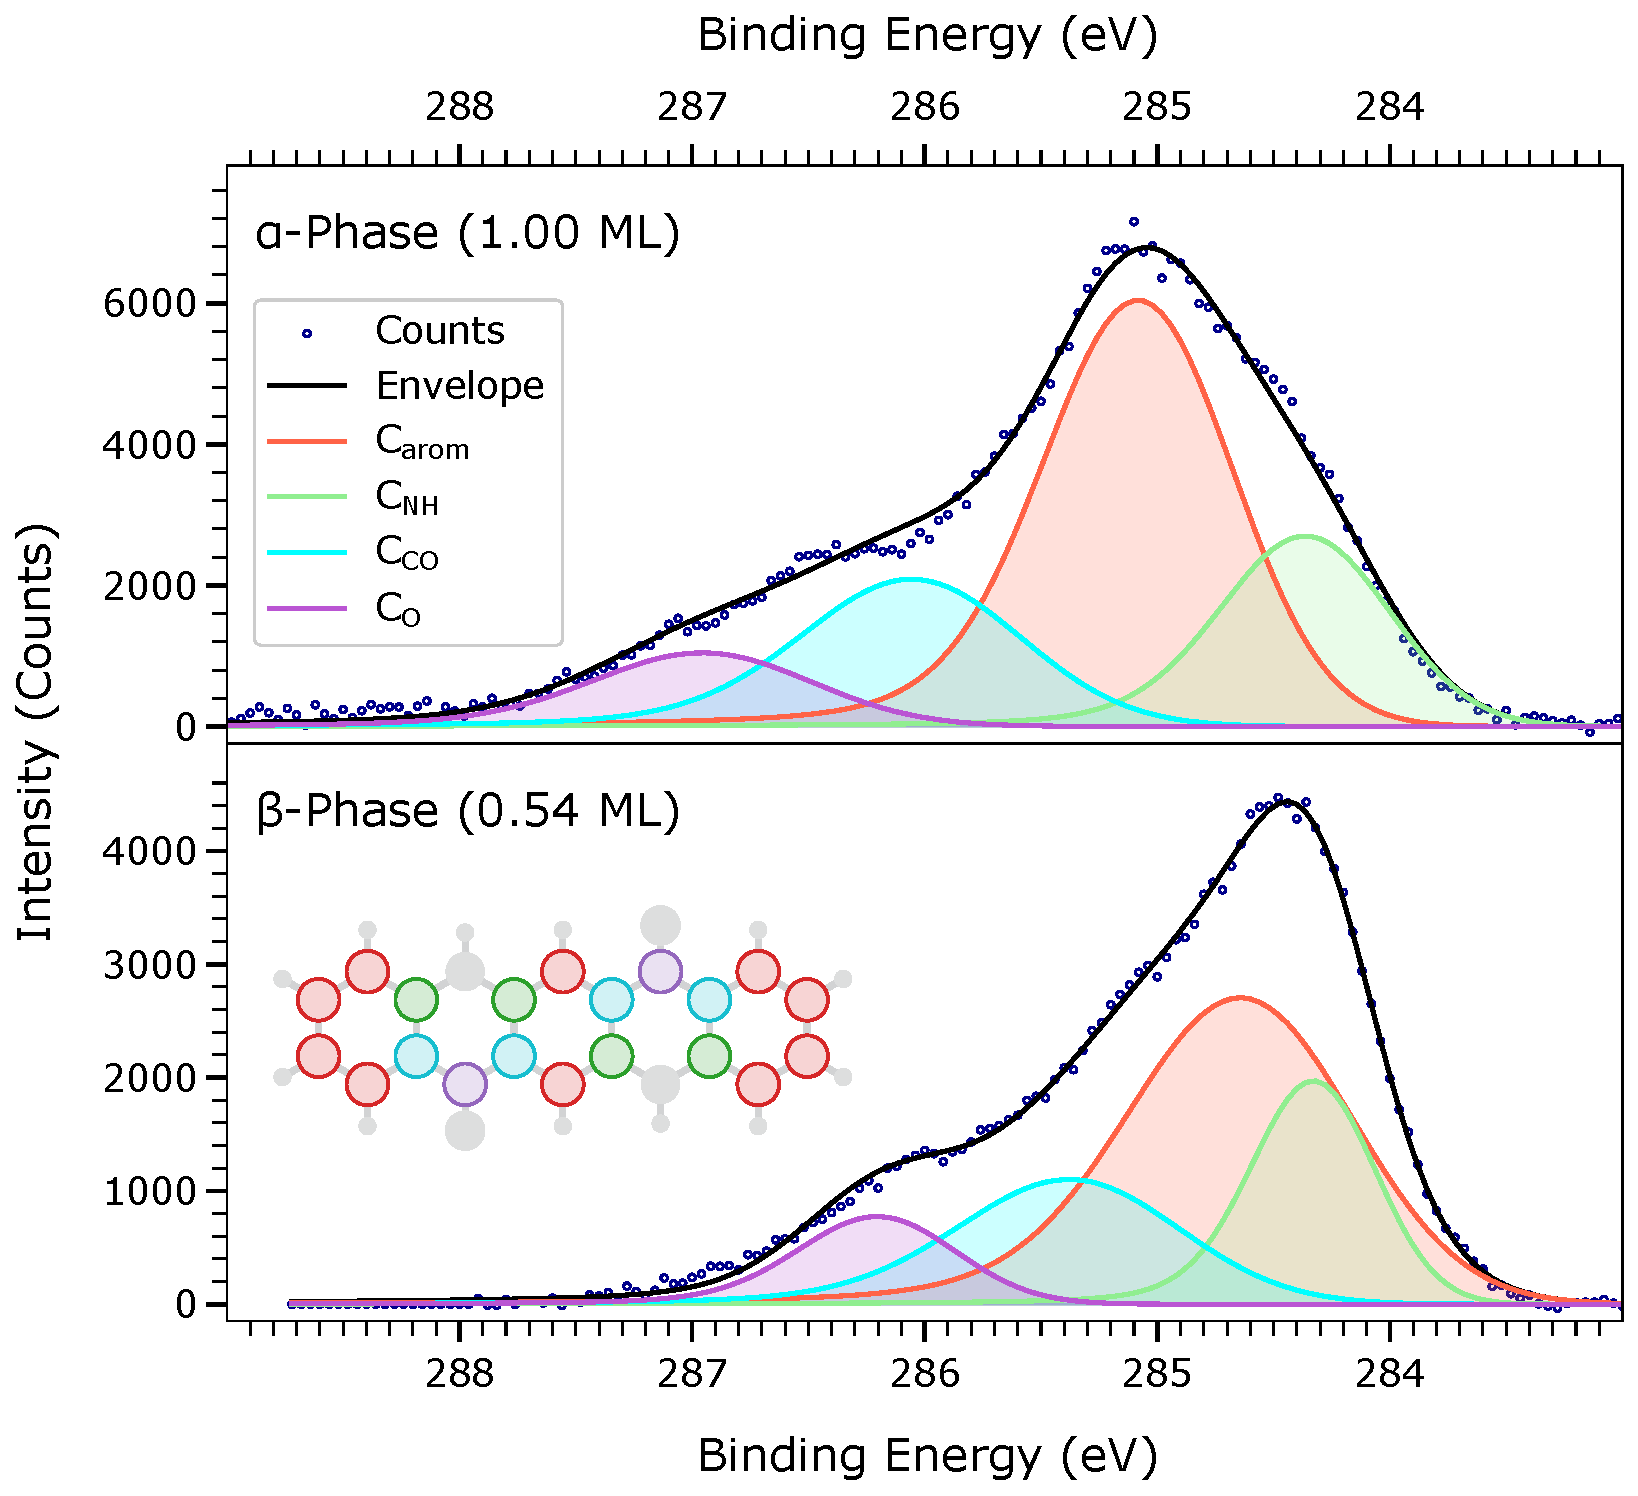
\includegraphics[width=\textwidth]{images/XPS/C1s-Phases.pdf}
    \caption{Comparison of the C1s \ac{XPS} spectra of \ac{QA} on the Ag(100) surface in the $\alpha$-phase and in the $\beta$-phase with the counts (blue circles), $\mathrm{C_{arom}}$ (red), $\mathrm{C_{NH}}$ (green), $\mathrm{C_{CO}}$ (lightblue), $\mathrm{C_{O}}$ (purple) and the resulting envelope (black). The used fit parameters are summarized in \autoref{tab:XPS-C1s-fit}.}
    \label{fig:XPS-C1s-alpha}
\end{figure}

\autoref{fig:XPS-C1s-alpha} shows a clear shift of all peaks to lower \ac{BE} when going from the $\alpha$-phase to the $\beta$-phase. The $\mathrm{C_{arom}}$ peak shifts from 295.00~\si{eV} in the $\alpha$-phase to 284.54~\si{eV} in the $\beta$-phase, resulting in a shift of 0.46~\si{eV}. The $\mathrm{C_{CO}}$ peak shifts by 0.68~\si{eV} from 285.96~\si{eV} to 285.28~\si{eV}, while the $\mathrm{C_{O}}$ peak shows a shift of 0.73~\si{eV} from 286.86~\si{eV} to 286.13~\si{eV}. In total, these 3 peaks show similar shifts of approximately 0.6~\si{eV}. 

The $\mathrm{C_{NH}}$ peak exhibits a different behavior, as it only shifts by 0.02~\si{eV} from 284.29~\si{eV} in the $\alpha$-phase to 284.27~\si{eV} in the $\beta$-phase. The \ac{BE} shift of the $\mathrm{C_{NH}}$ peak indicates a very unique change in the chemical environment during the phase transition compared to the other C atoms.

The \ac{FWHM} of the peaks also changes form the $\alpha$- to the $\beta$-phase. The $\mathrm{C_{arom}}$ peak broadens from 0.95~\si{eV} in the $\alpha$-phase to 1.13~\si{eV} in the $\beta$-phase. The \ac{FWHM} of the $\mathrm{C_{CO}}$ peak shows a almost no change, while the $\mathrm{C_{O}}$ peak narrows from a \ac{FWHM} of 1.1~\si{eV} to 0.79~\si{eV}. The \ac{FWHM} of the $\mathrm{C_{NH}}$ peak significantly decreases from 0.85~\si{eV} in the $\alpha$-phase to 0.62~\si{eV} in the $\beta$-phase.

The fit parameters for the C1s \ac{XPS} spectra of \ac{QA} on the Ag(100) surface in the $\alpha$- and $\beta$-phase are summarized in \autoref{tab:XPS-C1s-fit}.

\begin{table}[H]
	\centering
	\caption{\Ac{BE}, \ac{FWHM} and area ratio for the different peaks of the C1s \ac{XPS} spectra of \ac{QA} on the Ag(100) surface in the $\alpha$- and $\beta$-phase.}
	\begin{tabular}{@{}ccccc@{}} \toprule
		 & peak & \ac{BE} (eV) & \ac{FWHM} (eV) & area ratio \\
		\midrule
		$\alpha$-phase & $\mathrm{C_{arom}}$ & 285.00 & 0.95 & 10 \\
		& $\mathrm{C_{NH}}$ & 284.29 & 0.85 & 4 \\
		& $\mathrm{C_{CO}}$ & 285.96 & 1.1 & 4 \\ 
		& $\mathrm{C_{O}}$ & 286.86 & 1.1 & 2 \\
        \midrule
		$\beta$-phase & $\mathrm{C_{arom}}$ & 284.54 & 1.13 & 10 \\
		& $\mathrm{C_{NH}}$ & 284.27 & 0.62 & 4 \\
		& $\mathrm{C_{CO}}$ & 285.28 & 1.11 & 4 \\ 
		& $\mathrm{C_{O}}$ & 286.13 & 0.79 & 2 \\
		\bottomrule
	\end{tabular}
	\label{tab:XPS-C1s-fit}
\end{table}

The values for the \ac{BE} and the \ac{FWHM} can be compared to literature values of similar molecules on metal surfaces. For example, \ac{PTCDA} on the Ag(100) surface shows different peaks for the following C atoms: $\mathrm{C_{C-C}}$, $\mathrm{C_{C-H}}$, and $\mathrm{C_{funct}}$. The $\mathrm{C_{C-C}}$ peak with a \ac{BE} of 284.07~\si{eV} and the $\mathrm{C_{C-C}}$ peak with a \ac{BE} of 284.39~\si{eV} for \ac{PTCDA} are comparable to the $\mathrm{C_{arom}}$ peak for \ac{QA}. The \ac{BE} for \ac{PTCDA} is similar to the \ac{BE} for \ac{QA}, but slightly lower by approximately 0.2-0.5~\si{eV}.\autocite{Bauer2014}

The $\mathrm{C_{C-CO}}$ peak for \ac{PTCDA} with a \ac{BE} of 284.99~\si{eV} exhibits a 0.6~\si{eV} higher \ac{BE} than the $\mathrm{C_{C-H}}$ peak and a 0.72~\si{eV} higher \ac{BE} than the $\mathrm{C_{C-C}}$ peak.\autocite{Bauer2014} This finding is similar to the \ac{BE} difference between the $\mathrm{C_{arom}}$ peak and the $\mathrm{C_{CO}}$ peak for \ac{QA} in the $\alpha$-phase (0.96~\si{eV}) and in the $\beta$-phase (0.74~\si{eV}).

The $\mathrm{C_{funct}}$ peak for \ac{PTCDA} with a \ac{BE} of 286.96~\si{eV} shows a 2.9~\si{eV} higher \ac{BE} than the $\mathrm{C_{C-C}}$ peak and a 2.6~\si{eV} higher \ac{BE} than the $\mathrm{C_{C-H}}$ peak.\autocite{Bauer2014} This differences in the \ac{BE} are slightly lower than the \ac{BE} difference between the $\mathrm{C_{arom}}$ peak and the $\mathrm{C_{O}}$ peak for \ac{QA} in the $\alpha$-phase (1.86~\si{eV}) and in the $\beta$-phase (1.59~\si{eV}).
However, the general trend of increasing \ac{BE} for C atoms bonded to more electronegative atoms is the same for both molecules.

Another comparable molecule is indigo due to the presence of the aromatic ring, the N atoms, and the O atoms. The C1s \ac{XPS} spectrum of indigo in \ac{UHV} but on a non-reactive MoS$_2$ substrate shows 2 different peaks and two shake-up features.\autocite{Michels2021} The main peak contains the C atoms from the aromatic rings and has a \ac{BE} of approximately 286~\si{eV}. The second peak at a higher \ac{BE} of approximately 287.5~\si{eV} corresponds to the C atoms bonded to the N and O atoms.\autocite{Michels2021}

The relative position of the peaks is similar to the C1s \ac{XPS} spectra of \ac{QA} on the Ag(100) surface, where the $\mathrm{C_{arom}}$ peak has a lower \ac{BE} than the $\mathrm{C_{CO}}$ and $\mathrm{C_{O}}$ peaks. However, the absolute \ac{BE} values for indigo are approximately 1-2~\si{eV} higher than for \ac{QA}, which can be explained by the very different substrate effects and molecular structures.


\subsection{Fit model for the NIXSW analysis in the \texorpdfstring{$\beta$}{beta}-phase}

The C1s \ac{XPS} spectra of \ac{QA} on the Ag(100) surface in the $\beta$-phase were also fitted with a model containing only 3 peaks, where the C atoms from the $\mathrm{C_{NH}}$ peak are included in the $\mathrm{C_{arom}}$ peak. This fit model was used for the \ac{NIXSW} analysis in the \autoref{chap:C1s-NIXSW}, because the $\mathrm{C_{NH}}$ peak shows only a very small shift in its \ac{BE} during the phase transition and therefore strongly overlaps with the $\mathrm{C_{arom}}$ peak. This leads to a large uncertainty in the fit parameters for the \ac{NIXSW} spectra of the $\mathrm{C_{NH}}$ peak in the $\beta$-phase. The resulting fit is shown in \autoref{fig:XPS-C1s-3peaks}.

\begin{figure}[H]
    \centering
    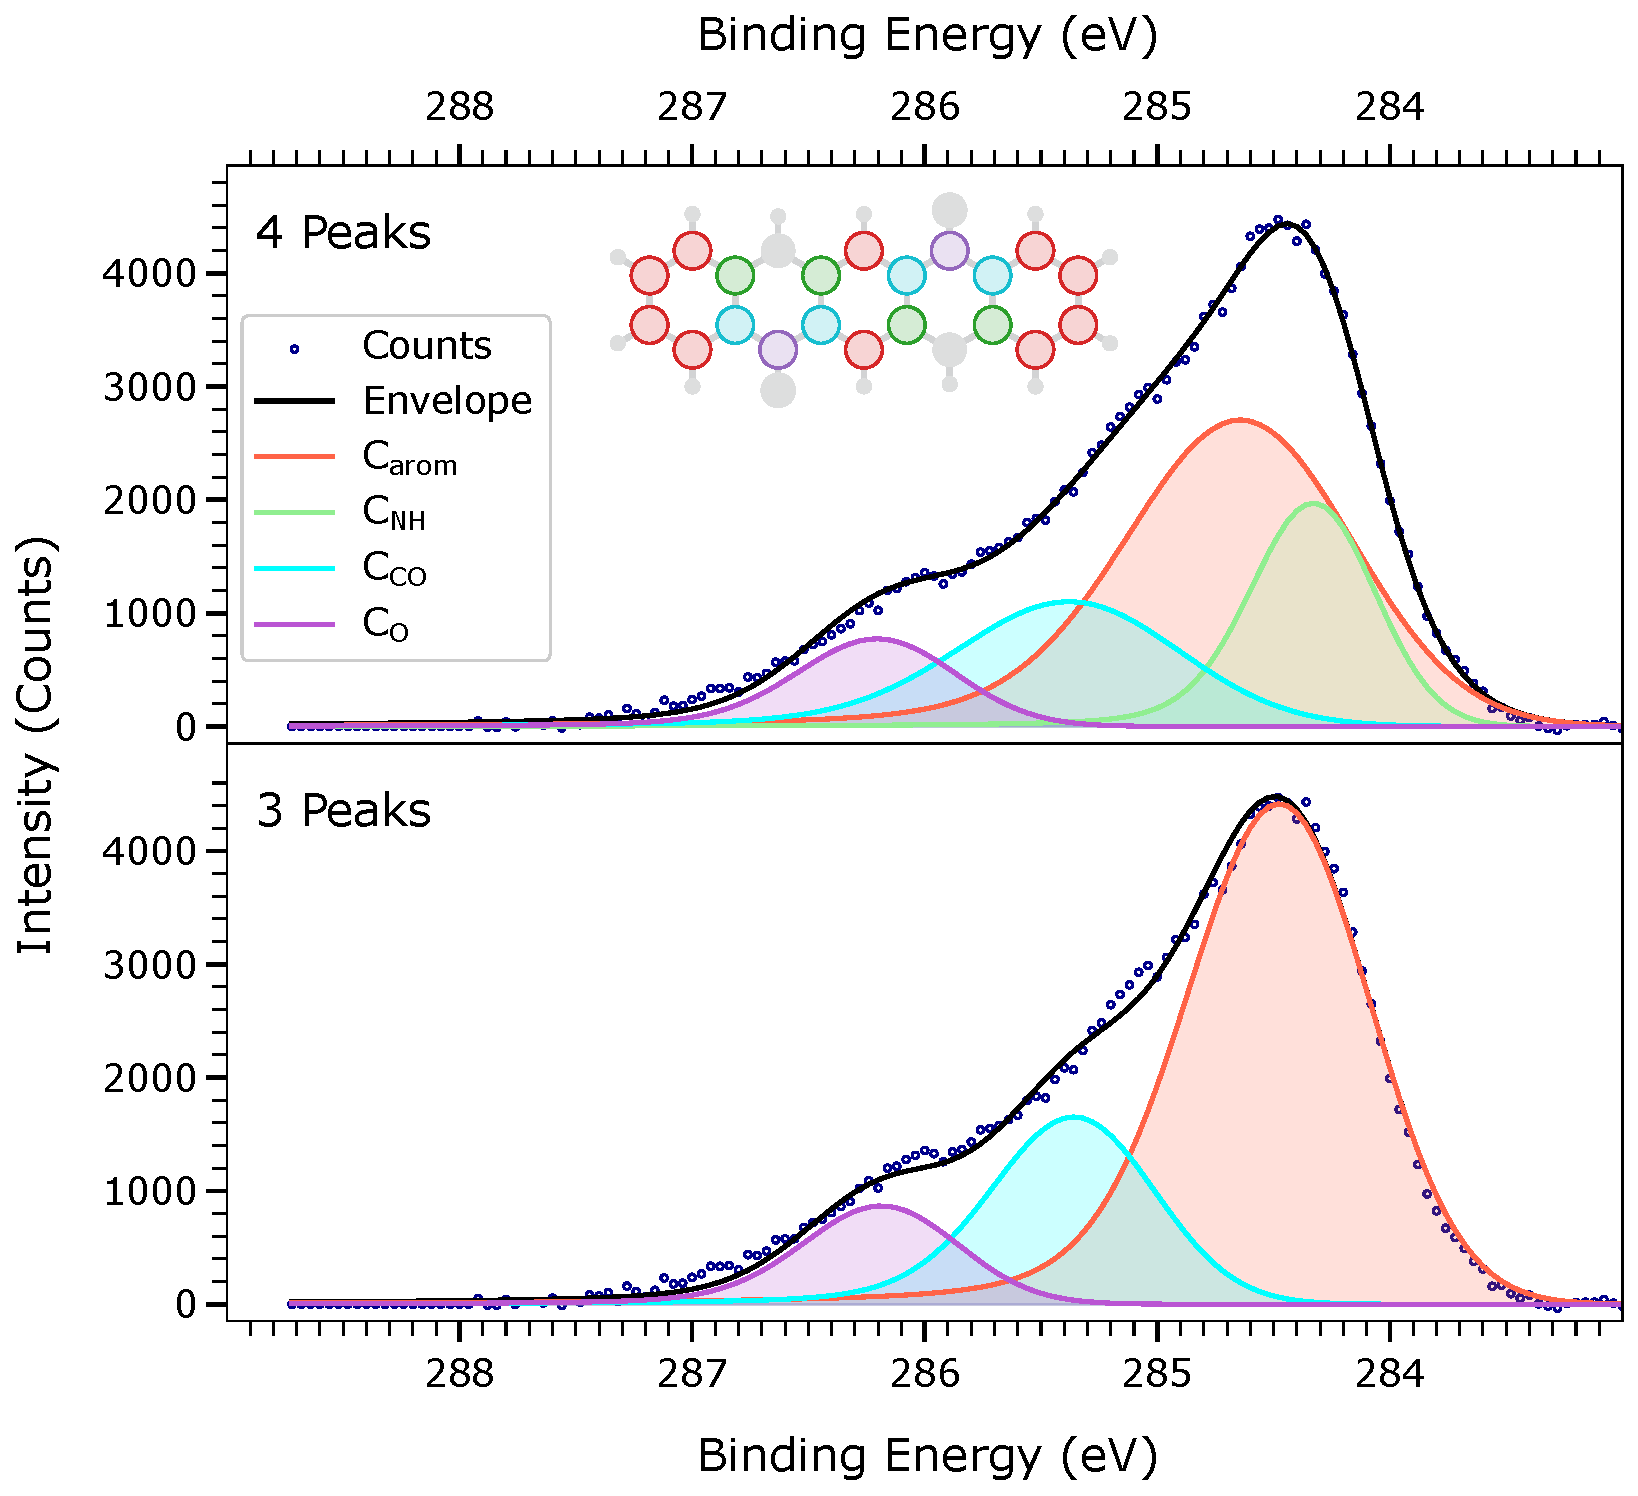
\includegraphics[width=\textwidth]{images/XPS/C1s-FitModel-NIXSW.pdf}
    \caption{Comparison of the C1s \ac{XPS} spectra of \ac{QA} on the Ag(100) surface in the $\beta$-phase with 4 and 3 peaks fitted. The figure contains the counts (blue circles), $\mathrm{C_{arom}}$ (red), $\mathrm{C_{NH}}$ (green), $\mathrm{C_{CO}}$ (lightblue), $\mathrm{C_{O}}$ (purple) and the resulting envelope (black). The $\mathrm{C_{NH}}$ peak is omitted in the fit with 3 peaks. The used fit parameters are summarized in \autoref{tab:XPS-C1s-fit-3peaks}.}
    \label{fig:XPS-C1s-3peaks}
\end{figure}

The fit parameters for the C1s \ac{XPS} spectra of \ac{QA} on the Ag(100) surface in the $\beta$-phase with both fit models are summarized in \autoref{tab:XPS-C1s-fit-3peaks}.

\begin{table}[H]
	\centering
	\caption{\Ac{BE}, \ac{FWHM} and area ratio for the different peaks of the C1s \ac{XPS} spectra of \ac{QA} on the Ag(100) surface in the $\beta$-phase with 4 and 3 peaks fitted.}
	\begin{tabular}{@{}ccccc@{}} \toprule
		 & peak & \ac{BE} (eV) &  \ac{FWHM} (eV) & area ratio \\
		\midrule
		$\beta$-phase - 4 peaks & $\mathrm{C_{arom}}$ & 284.54 & 1.13 & 10 \\
		& $\mathrm{C_{NH}}$ & 284.27 & 0.62 & 4 \\
		& $\mathrm{C_{CO}}$ & 285.28 & 1.11 & 4 \\ 
		& $\mathrm{C_{O}}$ & 286.13 & 0.79 & 2 \\
        \midrule
		$\beta$-phase - 3 peaks & $\mathrm{C_{arom}}+\mathrm{C_{NH}}$ & 284.39 & 0.92 & 14 \\
		& $\mathrm{C_{CO}}$ & 285.29 & 0.82 & 4 \\ 
		& $\mathrm{C_{O}}$ & 286.12 & 0.78 & 2 \\
		\bottomrule
	\end{tabular}
	\label{tab:XPS-C1s-fit-3peaks}
\end{table}

As seen in \autoref{fig:XPS-C1s-3peaks} and \autoref{tab:XPS-C1s-fit-3peaks}, both fit models describe the experimental data very well. The \ac{FWHM} of the combined $\mathrm{C_{arom}}+\mathrm{C_{NH}}$ peak is 0.92~\si{eV}, which is in between the \ac{FWHM} of the individual peaks (1.13~\si{eV} and 0.62~\si{eV}). The \ac{BE} of the combined peak is 284.39~\si{eV}, which is also in between the individual \ac{BE} values of 284.54~\si{eV} and 284.27~\si{eV}. The area ratio of the combined peak is 14, which is the sum of the individual area ratios of 10 and 4.

The $\mathrm{C_{CO}}$ and $\mathrm{C_{O}}$ peaks show almost no change in their \ac{BE} when comparing both fit models. Nevertheless, the \ac{FWHM} of the $\mathrm{C_{CO}}$ peak decreases from 1.11~\si{eV} to 0.82~\si{eV} when using the fit model with 3 peaks, but the \ac{FWHM} of the $\mathrm{C_{O}}$ peak remains unchanged. The change in the \ac{FWHM} of the $\mathrm{C_{CO}}$ peak can be explained by the larger seperation with respect to the combined $\mathrm{C_{arom}}+\mathrm{C_{NH}}$ peak compared to the individual $\mathrm{C_{arom}}$ peak.

\subsection{C1s XPS spectra for the Multilayer}

In addition to the C1s \ac{XPS} spectra of \ac{QA} on the Ag(100) surface in the $\alpha$- and $\beta$-phase, a C1s \ac{XPS} spectrum of a \ac{QA} multilayer on the Ag(100) surface is compared to the preparation with a coverage of 1~\ac{ML} in \autoref{fig:C1s-XPS-multilayer}.

\begin{figure}[H]
	\centering
	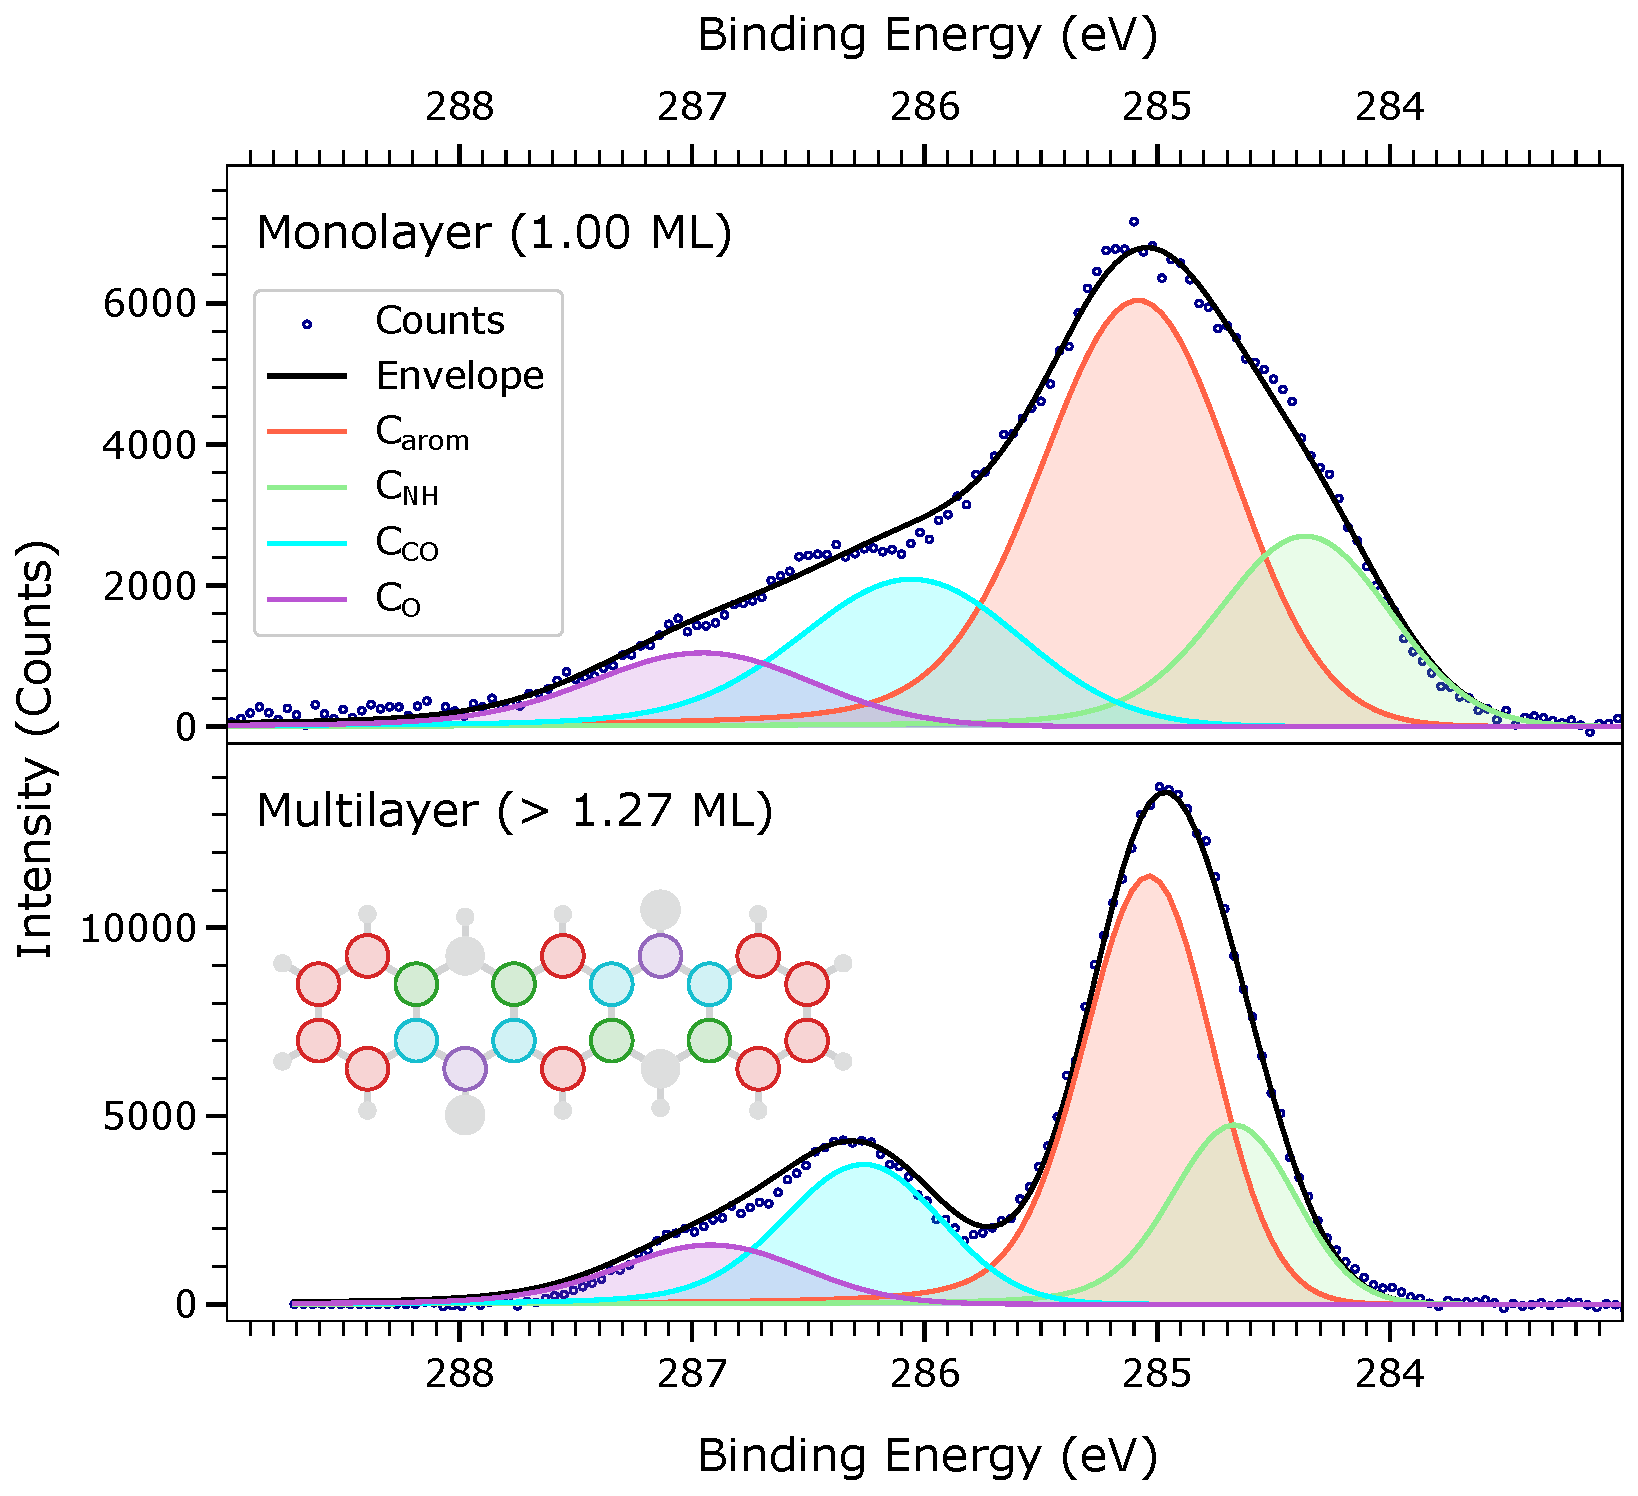
\includegraphics[width=\textwidth]{images/XPS/C1s-Multilayer.pdf}
	\caption{Comparison of the C1s \ac{XPS} spectra of \ac{QA} on the Ag(100) surface in the $\alpha$-phase for 1.00~\ac{ML} and 1.27~\ac{ML} coverage with the counts (blue circles), $\mathrm{C_{arom}}$ (red), $\mathrm{C_{NH}}$ (green), $\mathrm{C_{CO}}$ (lightblue), $\mathrm{C_{O}}$ (purple) and the resulting envelope (black). The used fit parameters are summarized in \autoref{tab:XPS-C1s-Multilayer-fit}.}
	\label{fig:C1s-XPS-multilayer}
\end{figure}

The C1s \ac{XPS} spectrum of the \ac{QA} multilayer was fitted with the same model as used for the $\alpha$-phase and the fit parameters are summarized in \autoref{tab:XPS-C1s-Multilayer-fit}.

\begin{table}[H]
	\centering
	\caption{\Ac{BE}, \ac{FWHM} and area ratio for the different peaks of the C1s \ac{XPS} spectra of \ac{QA} with a \ac{ML} and Multilayer coverage on the Ag(100) surface in the $\alpha$-phase.}
	\begin{tabular}{@{}ccccc@{}} \toprule
		 & peak & \ac{BE} (eV) & \ac{FWHM} (eV) & area ratio \\
		\midrule
		1.00~\ac{ML} & $\mathrm{C_{arom}}$ & 285.00 & 0.95 & 10 \\
		& $\mathrm{C_{NH}}$ & 284.29 & 0.85 & 4 \\
		& $\mathrm{C_{CO}}$ & 285.96 & 1.1 & 4 \\ 
		& $\mathrm{C_{O}}$ & 286.86 & 1.1 & 2 \\
        \midrule
		1.27~\ac{ML} & $\mathrm{C_{arom}}$ & 284.98 & 0.64 & 10 \\
		& $\mathrm{C_{NH}}$ & 284.61 & 0.61 & 4 \\
		& $\mathrm{C_{CO}}$ & 286.19 & 0.78 & 4 \\ 
		& $\mathrm{C_{O}}$ & 286.84 & 0.92 & 2 \\
		\bottomrule
	\end{tabular}
	\label{tab:XPS-C1s-Multilayer-fit}
\end{table}

As seen in \autoref{fig:C1s-XPS-multilayer} and \autoref{tab:XPS-C1s-Multilayer-fit}, the C1s \ac{XPS} spectrum of the \ac{QA} multilayer shows a very different shape compared to the 1~\ac{ML} preparation. The \ac{FWHM} of all peaks decreases by 0.2-0.3~\si{eV} from the monolayer to the multilayer. Nevertheless, the \ac{BE} of the $\mathrm{C_{arom}}$ and the $\mathrm{C_{O}}$ peak remain almost unchanged, while the other 2 peaks shift to higher \ac{BE} by approximately 0.3~\si{eV}.

This again can be compared to \ac{PTCDA} on the Ag(100) surface. The C1s \ac{XPS} spectrum of a \ac{PTCDA} multilayer on the Ag(100) surface shows also a shift of the $\mathrm{C_{C-C}}$, $\mathrm{C_{C-H}}$ and $\mathrm{C_{C-CO}}$ peaks to higher \ac{BE} by approximately 0.5-0.9~\si{eV}. The $\mathrm{C_{funct}}$ peak, however, shows an even larger shift to higher \ac{BE} by approximately 2~\si{eV}.\autocite{Bauer2014}

This trend is similar to the C1s \ac{XPS} spectra of \ac{QA} on the Ag(100) surface in the monolayer and multilayer, where the peaks show no or only a small increase of 0.3~\si{eV} in the \ac{BE} for C atoms. Nevertheless, the changes are not comparable in detail, because the molecular structures of \ac{QA} and \ac{PTCDA} are very different and the differences in the coverages of the compared spectra are not the same.


\newpage
\section{N1s XPS spectra}

The N1s \ac{XPS} spectra of \ac{QA} on the Ag(100) surface in the $\alpha$- and $\beta$-phase are shown in \autoref{fig:XPS-N1s-alpha}. The preparation are the same as for the C1s spectra, with a coverage of 1~\ac{ML} for the $\alpha$-phase and 0.54~\ac{ML} for the $\beta$-phase.

\begin{figure}[H]
    \centering
    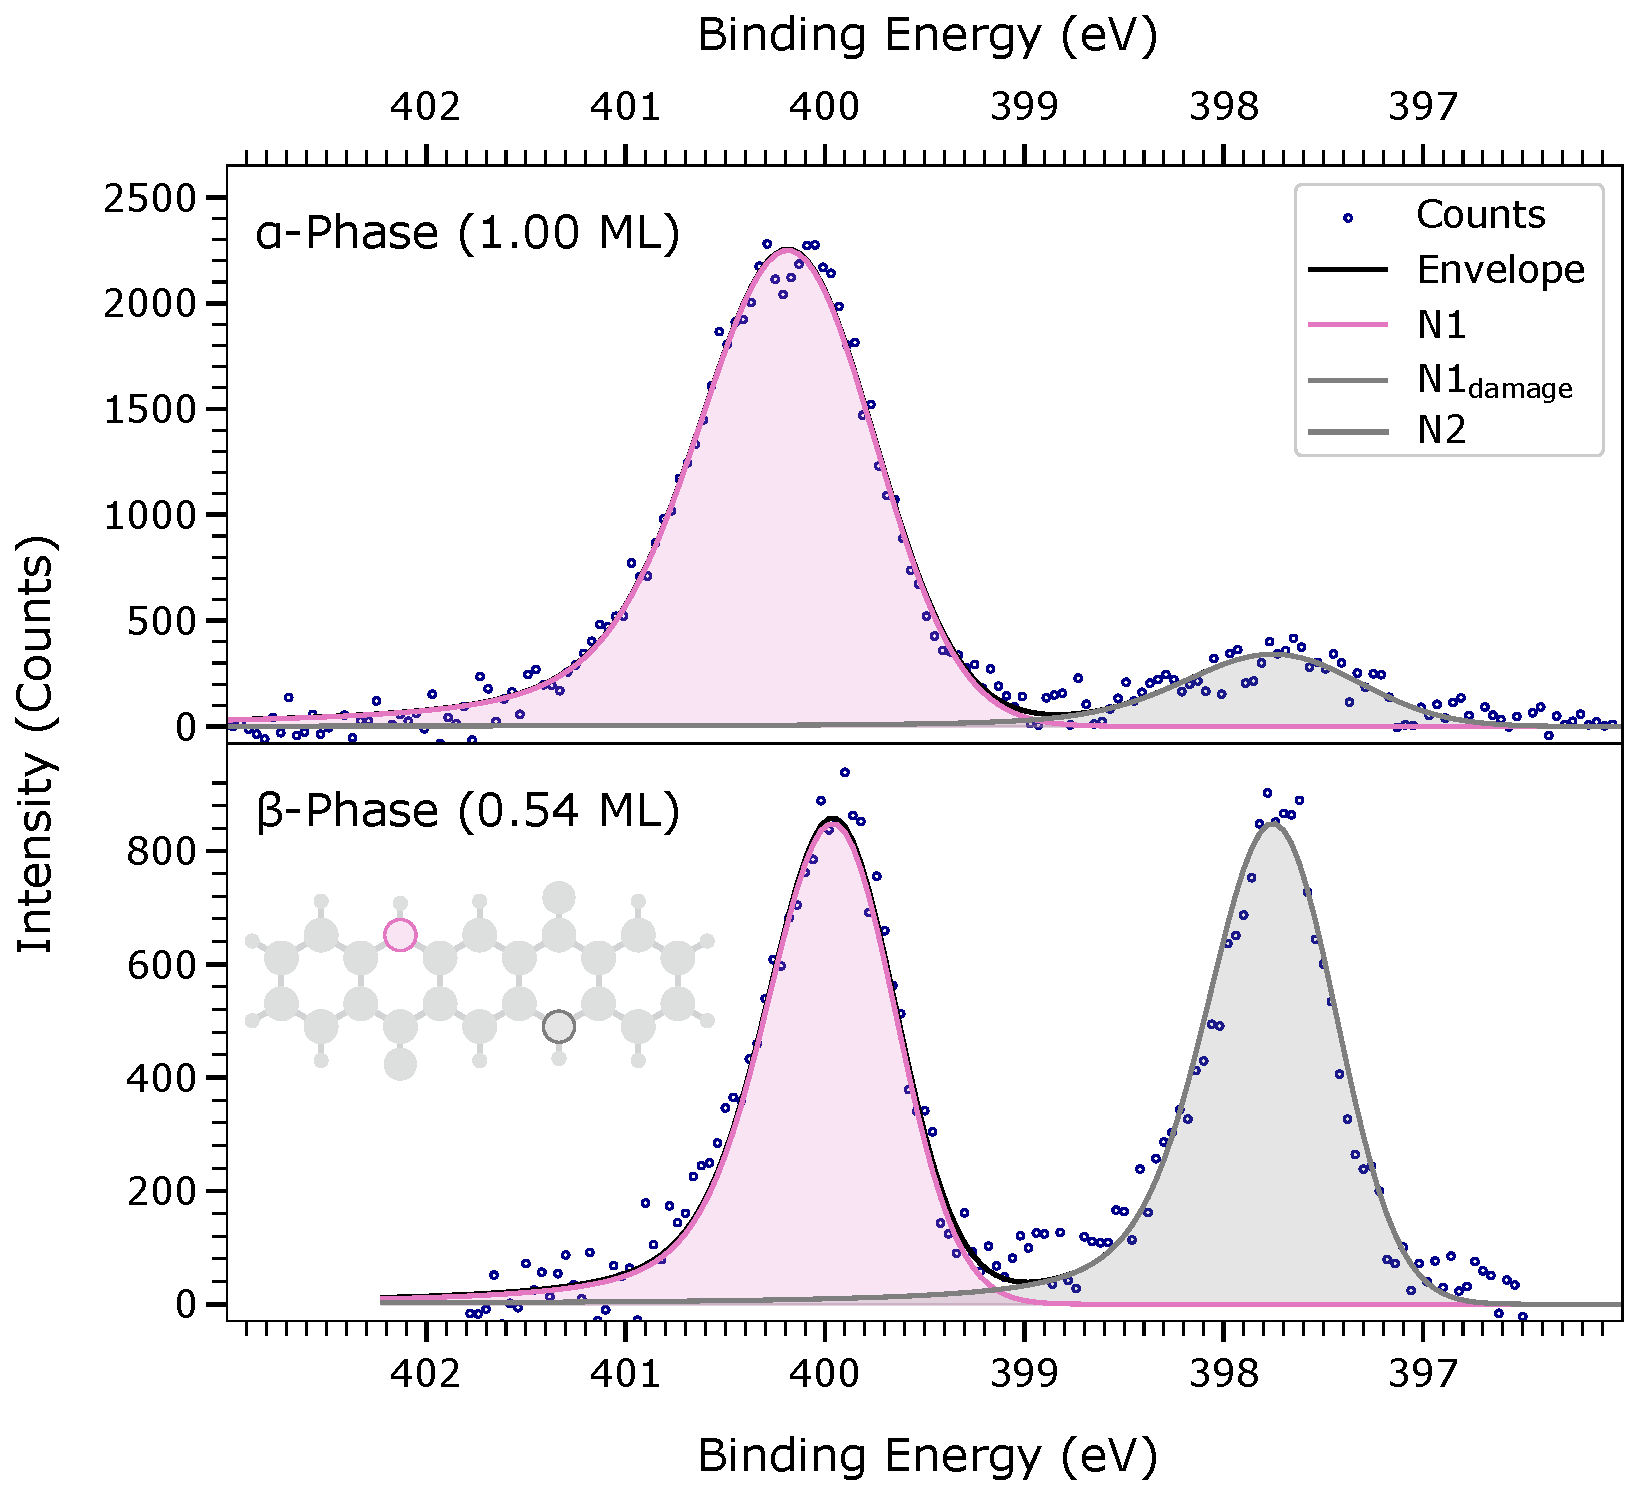
\includegraphics[width=\textwidth]{images/XPS/N1s-Phases.pdf}
    \caption{Comparison of the N1s \ac{XPS} spectra of \ac{QA} on the Ag(100) surface in the $\alpha$-phase and in the $\beta$-phase with the counts (blue circles), $\mathrm{N1}$ (purple), $\mathrm{N1_{damage}}$ (grey), $\mathrm{N2}$ (grey) and the resulting envelope (black). The used fit parameters are summarized in \autoref{tab:XPS-N1s-fit}.}
    \label{fig:XPS-N1s-alpha}
\end{figure}

The N1s \ac{XPS} spectra for both phases were fitted with different models, both having 2 peaks. The main component for the $\alpha$-phase is the $\mathrm{N1}$ peak, that originates from the 2 N atoms in the amine group forming hydrogen bonds with the O atoms with the carbonyl groups of the neighboring molecules. In addition, a second peak at lower \ac{BE} was observed, which is assigned to N atoms from the \ac{QA} molecules that have different chemical environments due to radiation damage ($\mathrm{N1_{damage}}$ peak). This peak is not related to the phase transition, but occurs due to prolonged exposure of the sample to the X-ray beam during the measurement. It was observed that the intensity of this peak changes for different measurements, which are shown in \autoref{fig:XPS-N1s-All}.

In the $\beta$-phase, there are also 2 peaks observed in the N1s \ac{XPS} spectrum. The main component is again the $\mathrm{N1}$ peak from one N atom in the amine group. However, the $\mathrm{N2}$ peak at lower \ac{BE} is assigned to a different chemical environment of one N atom in the $\beta$-phase. The detailed fit parameters are summarized in \autoref{tab:XPS-N1s-fit}.

\begin{table}[H]
	\centering
	\caption{\Ac{BE}, \ac{FWHM} and area ratio for the different peaks of the N1s \ac{XPS} spectra of \ac{QA} on the Ag(100) surface in the $\alpha$- and $\beta$-phase.}
	\begin{tabular}{@{}ccccc@{}} \toprule
		 & peak & \ac{BE} (eV) & \ac{FWHM} (eV) & area ratio \\
		\midrule
		$\alpha$-phase & $\mathrm{N1}$ & 400.05 & 1.02 & 1 \\
		& $\mathrm{N1_{damage}}$ & 397.66 & 1.02 & - \\
        \midrule
		$\beta$-phase & $\mathrm{N1}$ & 399.87 & 0.73 & 1 \\
		& $\mathrm{N2}$ & 397.66 & 0.73 & 1 \\
		\bottomrule
	\end{tabular}
	\label{tab:XPS-N1s-fit}
\end{table}

As seen in \autoref{fig:XPS-N1s-alpha} and \autoref{tab:XPS-N1s-fit}, the N1s \ac{XPS} spectrum of the $\beta$-phase shows only a minor change of 0.18~\si{eV} in the \ac{BE} of the $\mathrm{N1}$ peak. In contrast to the $\alpha$-phase, the $\beta$-phase exhibits a second peak ($\mathrm{N2}$) with the same area as the main peak, which indicates that both N atoms in the amine group have different chemical environments in the $\beta$-phase. The \ac{BE} of the $\mathrm{N2}$ peak is 397.66~\si{eV}, which is the same as the $\mathrm{N1_{damage}}$ peak in the $\alpha$-phase. This indicates that the chemical environment of one N atom in the $\beta$-phase is similar to the damaged N atoms in the $\alpha$-phase.

Furthermore, the \ac{FWHM} of both peaks decreases from 1.02~\si{eV} in the $\alpha$-phase to 0.73~\si{eV} in the $\beta$-phase, indicating a more uniform chemical environment for both N atoms in the amine group in the $\beta$-phase. 

The \ac{BE} of the N1s \ac{XPS} spectra of \ac{QA} on the Ag(100) surface can also be compared to literature values of similar molecules on metal surfaces. For example, the N1s \ac{XPS} spectrum of pyridine shows a peak at a \ac{BE} of approximately 400.18~\si{eV}.\autocite{Bagus2025}  Another example is 6,6'-dibromoindigo, that also shows a N1s peak at a \ac{BE} of 399.9~\si{eV}.\autocite{Xu2024} Both literature values are very similar to the \ac{BE} of the $\mathrm{N1}$ peak of \ac{QA} on the Ag(100) surface in both phases (400.05~\si{eV} and 399.87~\si{eV}).

The interpretation of the $\mathrm{N2}$ peak in the N1s \ac{XPS} spectrum of \ac{QA} on the Ag(100) surface in the $\beta$-phase more complex due to the very large change in its \ac{BE}. One possible explanation of this finding is the formation of an N-Ag bond. A similar behavior was observed for e.g. bis-(4-bromophenyl)amine on the Ag(111) surface.\autocite{Zhang2020} The formation of N-Ag bonds for bis-(4-bromophenyl)amine leads to a second N1s peak at a lower \ac{BE} of 397.1~\si{eV}, which is very similar to the \ac{BE} of the $\mathrm{N2}$ peak of \ac{QA} in the $\beta$-phase (397.66~\si{eV}).

However, the N-Ag bond formation in bis-(4-bromophenyl)amine occurs with the loss of the H atoms from the amine group.\autocite{Zhang2020} Similar deprotonation processes were also observed for other amine-containing molecules, e.g. glyphosate on different substrates.\autocite{Ruano2021} There, the N1s \ac{XPS} spectra show also a second peak at 2~\si{eV} lower \ac{BE} after the deprotonation of the amine group. In contrast to the aforementioned example, no N-Ag bond is formed. Another result of this study was, that the deprotonation also occurs when the molecules are exposed to the X-ray beam.\autocite{Ruano2021} Further studies of polyaniline films and polypyrrole show that the deprotonation of amine groups leads to a change in the \ac{BE} of the N1s peak of approximately 2~\si{eV} and that the peak of the deprotonated amine group is located at 397.7~\si{eV}.\autocite{Neoh1991,M.Mahat2015,Kang1991}

There are even more examples like n-butylamine on Au and Pt, where the deprotonation of the amine group leads to a second N1s peak at a 2~\si{eV} lower \ac{BE} than the main peak and a third peak at a 2~\si{eV} higher \ac{BE} corresponds to a protonated amine.\autocite{Adenier2004}

All of these literature examples show that the deprotonation of amine groups leads to a second N1s peak at approximately 2~\si{eV} lower \ac{BE} than the main peak. This is very similar to the N1s \ac{XPS} spectrum of \ac{QA} on the Ag(100) surface in the $\beta$-phase, where the $\mathrm{N2}$ peak is also located at a 2.2~\si{eV} lower \ac{BE} than the $\mathrm{N1}$ peak. Therefore, it is very likely that the formation of deprotonated amine groups occurs in the \ac{QA} monolayer in the $\beta$-phase. In addition, the deprotonation also occurs when the sample is exposed to the X-ray beam, which could explain why the $\mathrm{N1_{damage}}$ peak is located at the same \ac{BE} as the $\mathrm{N2}$ peak.


\subsection{Multilayer}

On top of the N1s \ac{XPS} spectra of \ac{QA} on the Ag(100) surface in the $\alpha$- and $\beta$-phase, a N1s \ac{XPS} spectrum of a \ac{QA} multilayer on the Ag(100) surface is compared to the $\alpha$-phase preparation with a coverage of 1~\ac{ML} in \autoref{fig:N1s-XPS-multilayer}.

\begin{figure}[H]
	\centering
	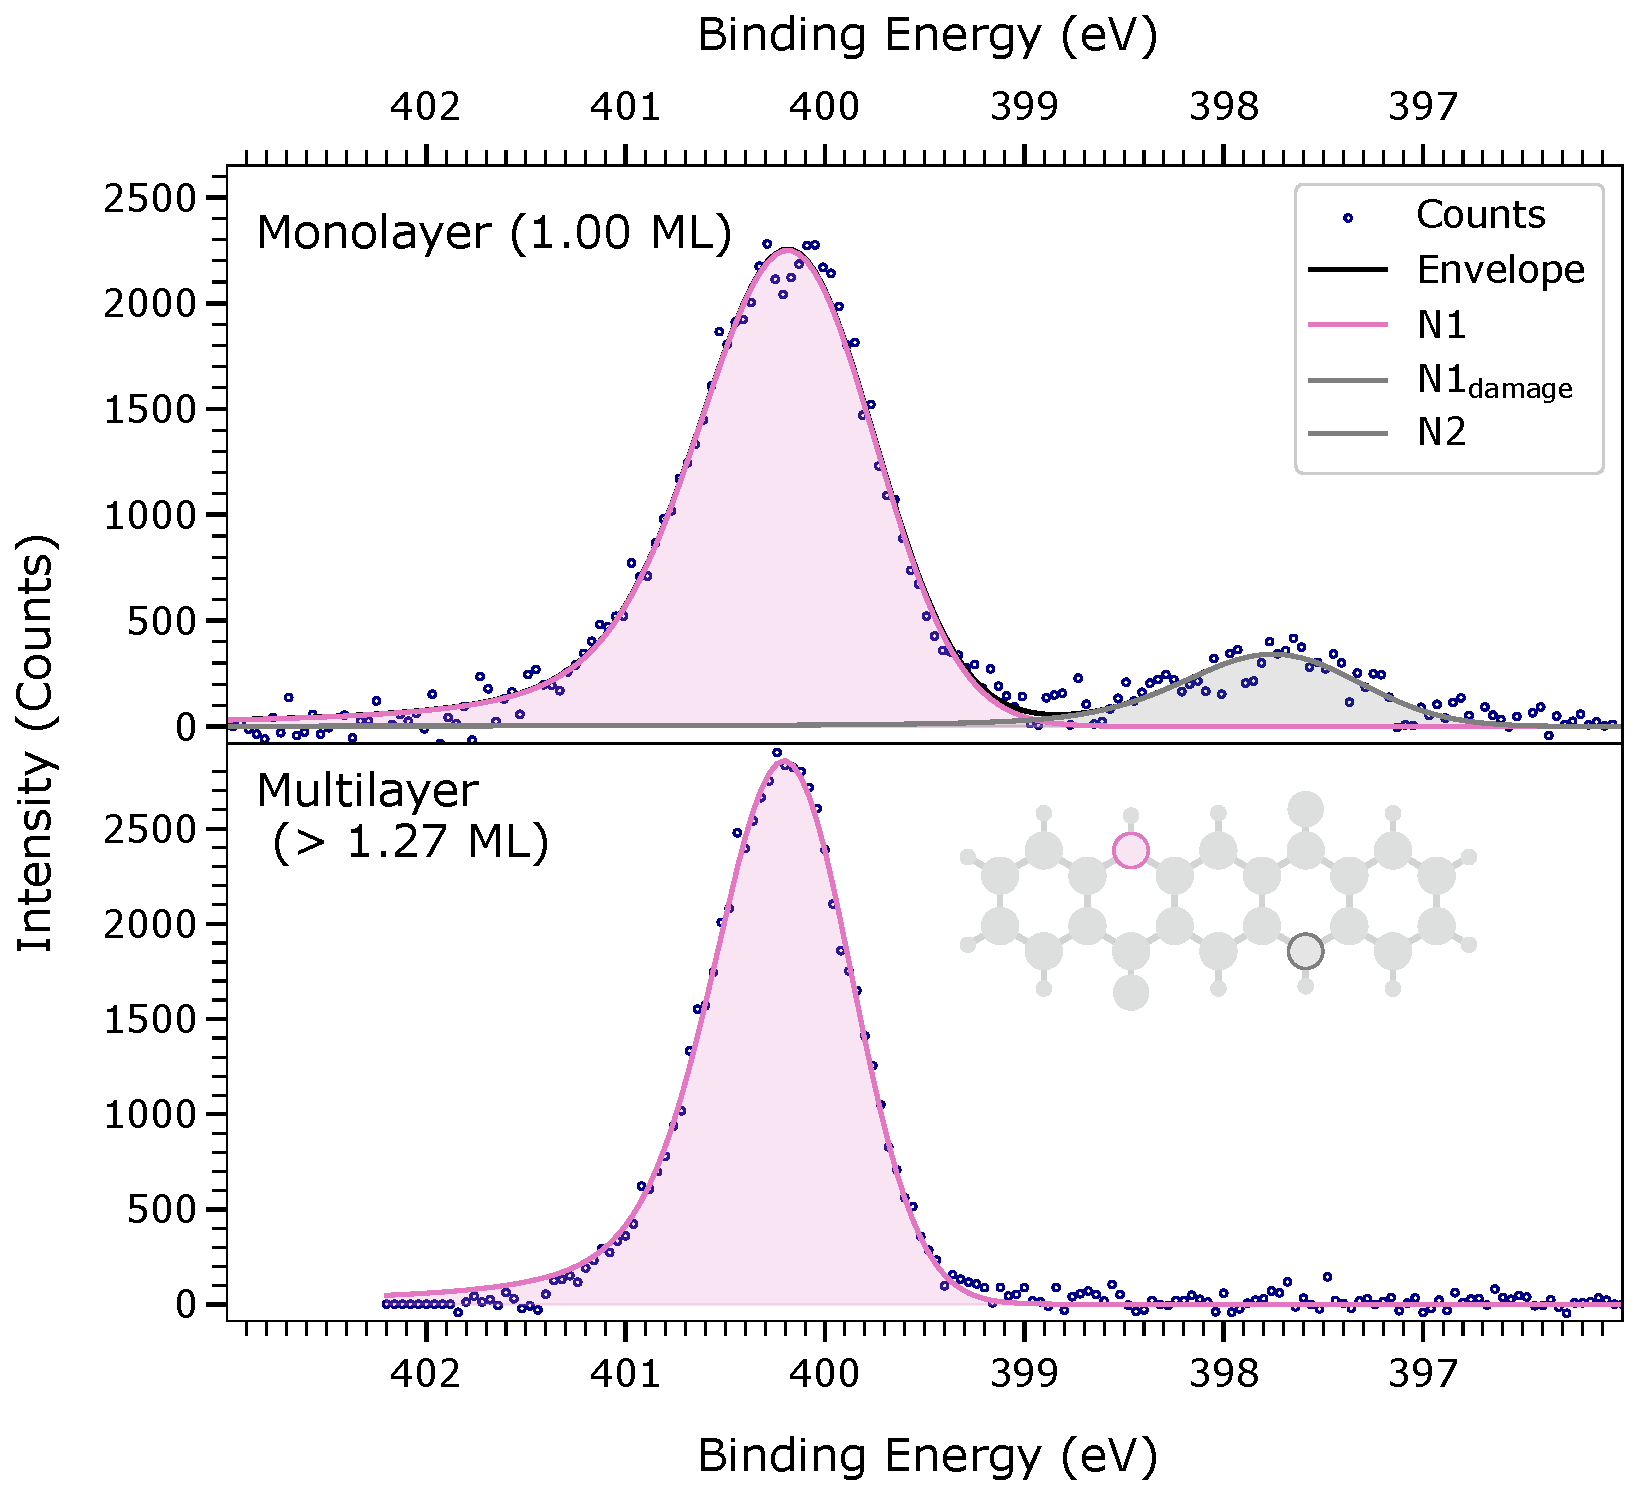
\includegraphics[width=\textwidth]{images/XPS/N1s-Multilayer.pdf}
	\caption{Comparison of the N1s \ac{XPS} spectra of \ac{QA} on the Ag(100) surface in the $\alpha$-phase for 1.00~\ac{ML} and 1.27~\ac{ML} coverage with the counts (blue circles), $\mathrm{N1}$ (purple), $\mathrm{N1_{damage}}$ (grey) and the resulting envelope (black). The used fit parameters are summarized in \autoref{tab:XPS-N1s-Multilayer-fit}.}
	\label{fig:N1s-XPS-multilayer}
\end{figure}

The corresponding fit parameters for the N1s \ac{XPS} spectra of \ac{QA} on the Ag(100) surface in the $\alpha$-phase with both coverages are summarized in \autoref{tab:XPS-N1s-Multilayer-fit}.

\begin{table}[H]
	\centering
	\caption{\Ac{BE}, \ac{FWHM} and area ratio for the different peaks of the N1s \ac{XPS} spectra of \ac{QA} with a \ac{ML} and Multilayer coverage on the Ag(100) surface in the $\alpha$-phase.}
	\begin{tabular}{@{}ccccc@{}} \toprule
		 & peak & \ac{BE} (eV) & \ac{FWHM} (eV) & area ratio \\
		\midrule
		1.00~\ac{ML} & $\mathrm{N1}$ & 400.05 & 1.02 & 1 \\
		& $\mathrm{N1_{damage}}$ & 397.66 & 1.02 & - \\
        \midrule
		1.27~\ac{ML} & $\mathrm{N1}$ & 400.10 & 0.79 & 1 \\
		\bottomrule
	\end{tabular}
	\label{tab:XPS-N1s-Multilayer-fit}
\end{table}

The N1s \ac{XPS} spectrum of the \ac{QA} multilayer exhibits only one peak, which corresponds to the $\mathrm{N1}$ peak from the amine group. The \ac{BE} of this peak is 400.10~\si{eV}, which is very similar to the 1~\ac{ML} preparation. However, the \ac{FWHM} decreases from 1.02~\si{eV} to 0.79~\si{eV}.

\newpage
\section{O1s XPS spectra}

The O1s \ac{XPS} spectra of \ac{QA} on the Ag(100) surface in the $\alpha$- and $\beta$-phase are shown in \autoref{fig:XPS-O1s-alpha}. The preparation are the same as for the C1s and N1s spectra, with a coverage of 1~\ac{ML} for the $\alpha$-phase and 0.54~\ac{ML} for the $\beta$-phase.

\begin{figure}[H]
    \centering
    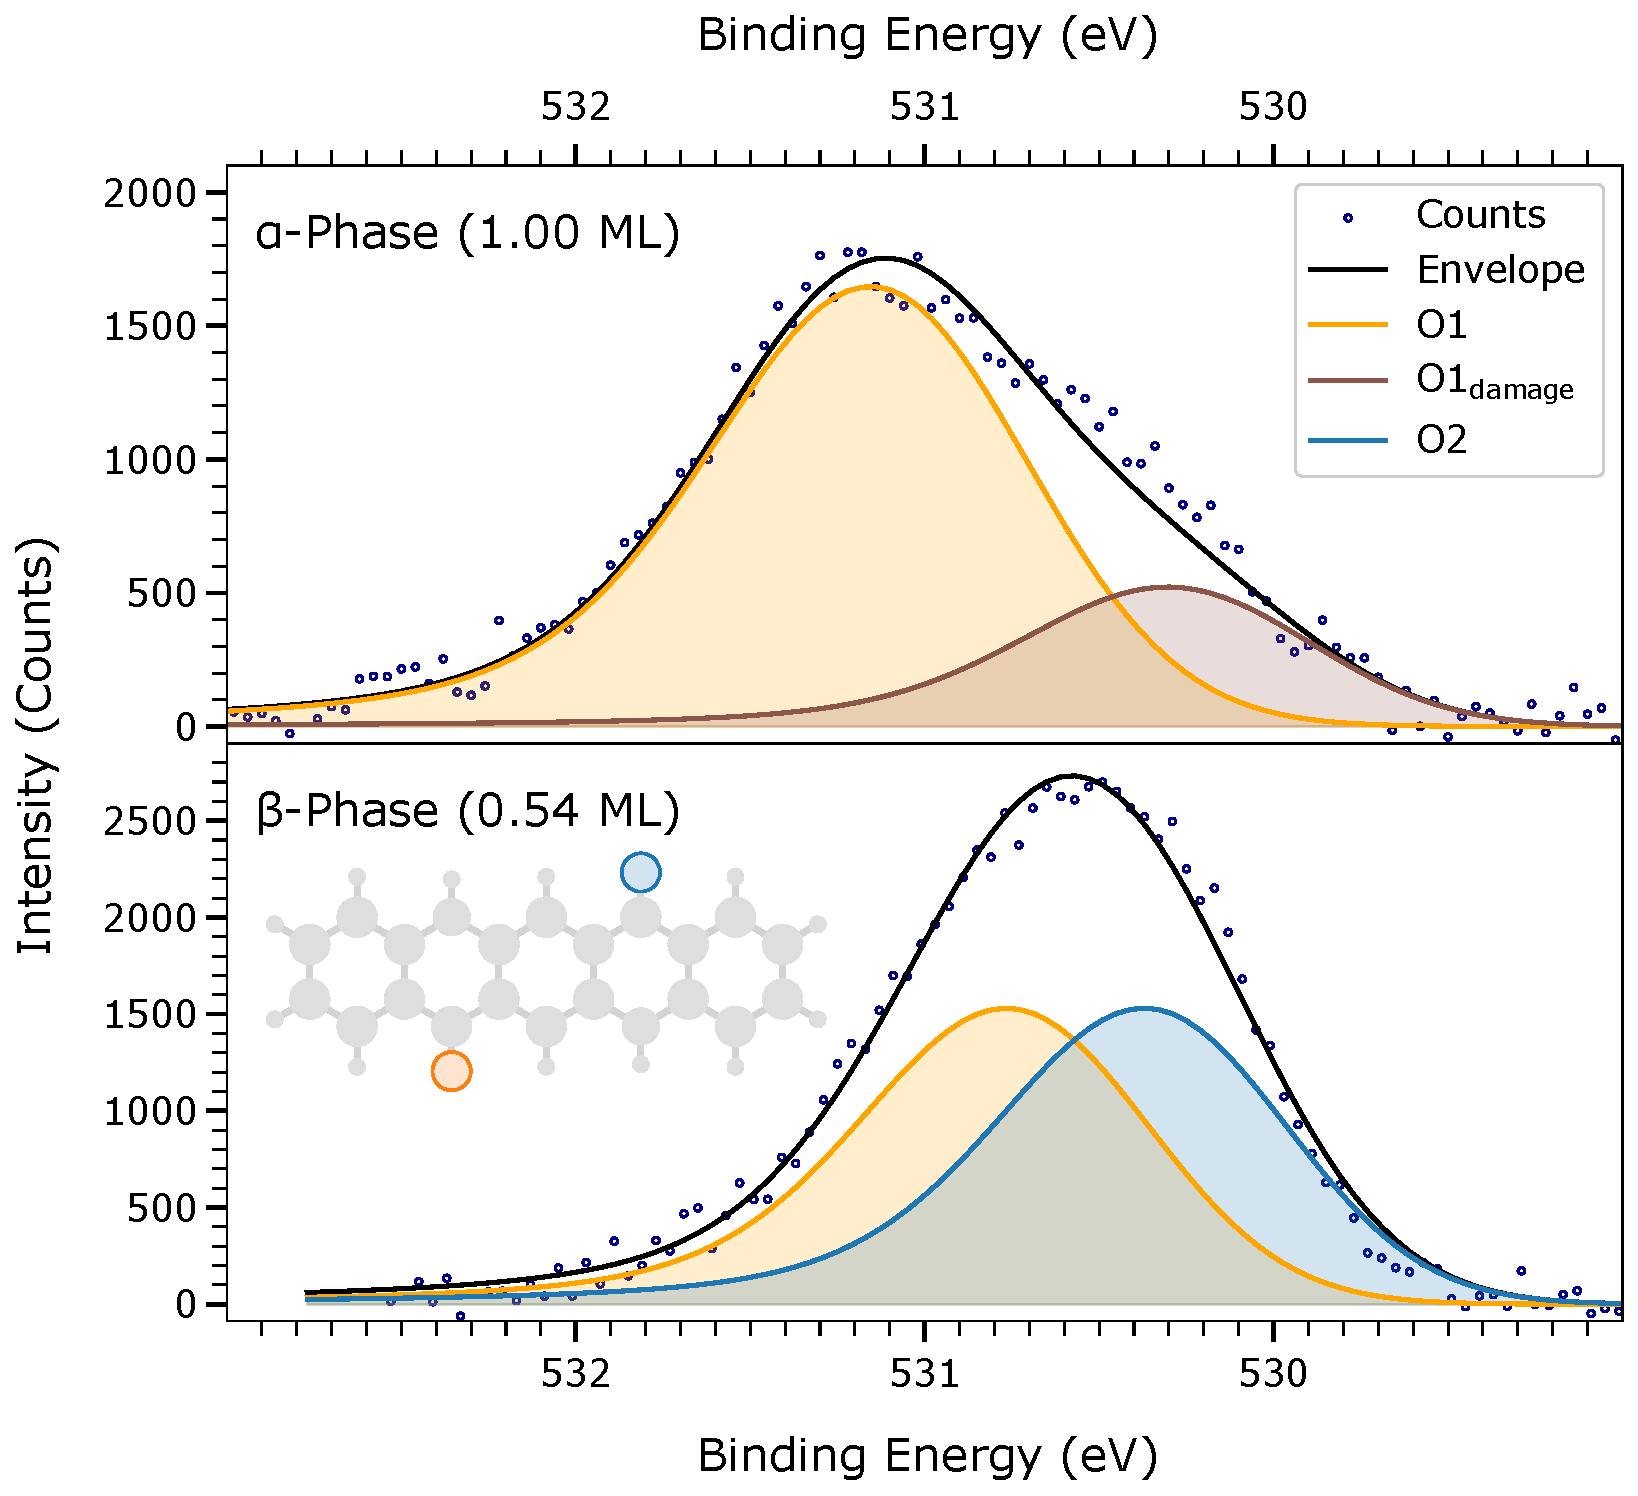
\includegraphics[width=\textwidth]{images/XPS/O1s-Phases.pdf}
    \caption{Comparison of the O1s \ac{XPS} spectra of \ac{QA} on the Ag(100) surface in the $\alpha$-phase and in the $\beta$-phase with the counts (blue circles), $\mathrm{O1}$ (yellow), $\mathrm{O1_{damage}}$ (brown), $\mathrm{O2}$ (blue) and the resulting envelope (black). The used fit parameters are summarized in \autoref{tab:XPS-O1s-fit}.}
    \label{fig:XPS-O1s-alpha}
\end{figure}

The O1s \ac{XPS} spectra for both phases were fitted with different models, both having 2 peaks as the N1s \ac{XPS} spectra. The 2 peaks of the O1s \ac{XPS} spectrum and the 2 peaks of the N1s \ac{XPS} spectrum are directly correlated, as both originate from functional groups that form hydrogen bonds with each other (amine and carbonyl group).

In the $\alpha$-phase, the main component is the $\mathrm{O1}$ peak, that originates from the 2 O atoms in the carbonyl groups forming hydrogen bonds with the N atoms in the amine groups of neighboring molecules. Similar to the N1s spectrum in the $\alpha$-phase, a second peak at lower \ac{BE} was observed, which is assigned to O atoms from the \ac{QA} molecules that have different chemical environments due to radiation damage ($\mathrm{O1_{damage}}$ peak). This peak is not related to the phase transition and only occurs due to exposure of the sample to the X-ray beam during the measurement. It was observed that the intensity of this peak changes for different measurements, which are shown in \autoref{fig:XPS-O1s-All}.

In the $\beta$-phase, there are also 2 peaks observed in the O1s \ac{XPS} spectrum. The main component is again the $\mathrm{O1}$ peak from one O atom in the carbonyl group. However, the $\mathrm{O2}$ peak at lower \ac{BE} is assigned to a different chemical environment of one O atom in the $\beta$-phase. Here, the $\mathrm{O1}$ peak can be assigned to the O atom that is involved in hydrogen bonding with the N atom in the amine group ($\mathrm{N1}$ peak), while the $\mathrm{O2}$ peak occurs from the O atom that is not involved in hydrogen bonding and thus positioned opposite to the N atoms of a neighboring molecule that correspond to the $\mathrm{N2}$ peak.

The detailed fit parameters are summarized in \autoref{tab:XPS-O1s-fit}.

\begin{table}[H]
	\centering
	\caption{\Ac{BE}, \ac{FWHM} and area ratio for the different peaks of the O1s \ac{XPS} spectra of \ac{QA} on the Ag(100) surface in the $\alpha$- and $\beta$-phase.}
	\begin{tabular}{@{}ccccc@{}} \toprule
		 & peak & \ac{BE} (eV) & \ac{FWHM} (eV) & area ratio \\
		\midrule
		$\alpha$-phase & $\mathrm{O1}$ & 531.02 & 1.05 & 1 \\
		& $\mathrm{O1_{damage}}$ & 530.18 & 0.95 & - \\
        \midrule
		$\beta$-phase & $\mathrm{O1}$ & 530.64 & 0.95 & 1 \\
		& $\mathrm{O2}$ & 530.25 & 0.95 & 1 \\
		\bottomrule
	\end{tabular}
	\label{tab:XPS-O1s-fit}
\end{table}

The \ac{BE} of the main $\mathrm{O1}$ peak shifts by 0.38~\si{eV} from 531.02~\si{eV} in the $\alpha$-phase to 530.64~\si{eV} in the $\beta$-phase. This shift is similar to the observed shifts for the N1s and C1s \ac{XPS} spectra, where the $\mathrm{N1}$ peak shifts by 0.18~\si{eV} and the C peaks shift by approximately 0.6~\si{eV}. The \ac{FWHM} of the $\mathrm{O1}$ peak decreases from 1.05~\si{eV} in the $\alpha$-phase to 0.95~\si{eV} in the $\beta$-phase. 

Again, the second peak in the $\beta$-phase ($\mathrm{O2}$) has the same area ratio as the main peak, indicating that both O atoms in the carbonyl groups have different chemical environments in the $\beta$-phase. The \ac{BE} of the $\mathrm{O2}$ peak is 530.25~\si{eV}, which is slightly lower than the $\mathrm{O1_{damage}}$ peak in the $\alpha$-phase (530.18~\si{eV}). This indicates that the chemical environment of one O atom in the $\beta$-phase is similar to the damaged O atoms in the $\alpha$-phase. The behaviour of the O1s peaks is thus directly correlated to the behaviour of the N1s peaks in both phases.

The O1s \ac{XPS} spectra of \ac{QA} on the Ag(100) surface can be compared to literature values of e.g. \ac{PTCDA}. The peak corresponding to the O atom from the keto group in \ac{PTCDA} has a \ac{BE} of 531.7~\si{eV}.\autocite{Bauer2014} Other O atoms in keto groups show also similar \ac{BE} values of 530.7-532.7~\si{eV}.\autocite{Lopez1991,Sparks1997,Schwaner1997} This is very similar to the \ac{BE} of the $\mathrm{O1}$ peak of \ac{QA} on the Ag(100) surface in the $\alpha$-phase and the $\beta$-phase (531.02~\si{eV} and 530.64~\si{eV}), confirming the plausibility of this assignment.


\subsection{O1s XPS spectra of the Multilayer}

Besides the O1s \ac{XPS} spectra of \ac{QA} on the Ag(100) surface in the $\alpha$- and $\beta$-phase, a O1s \ac{XPS} spectrum of a \ac{QA} multilayer on the Ag(100) surface is compared to the $\alpha$-phase preparation with a coverage of 1~\ac{ML} in \autoref{fig:O1s-XPS-multilayer}.

\begin{figure}[H]
	\centering
	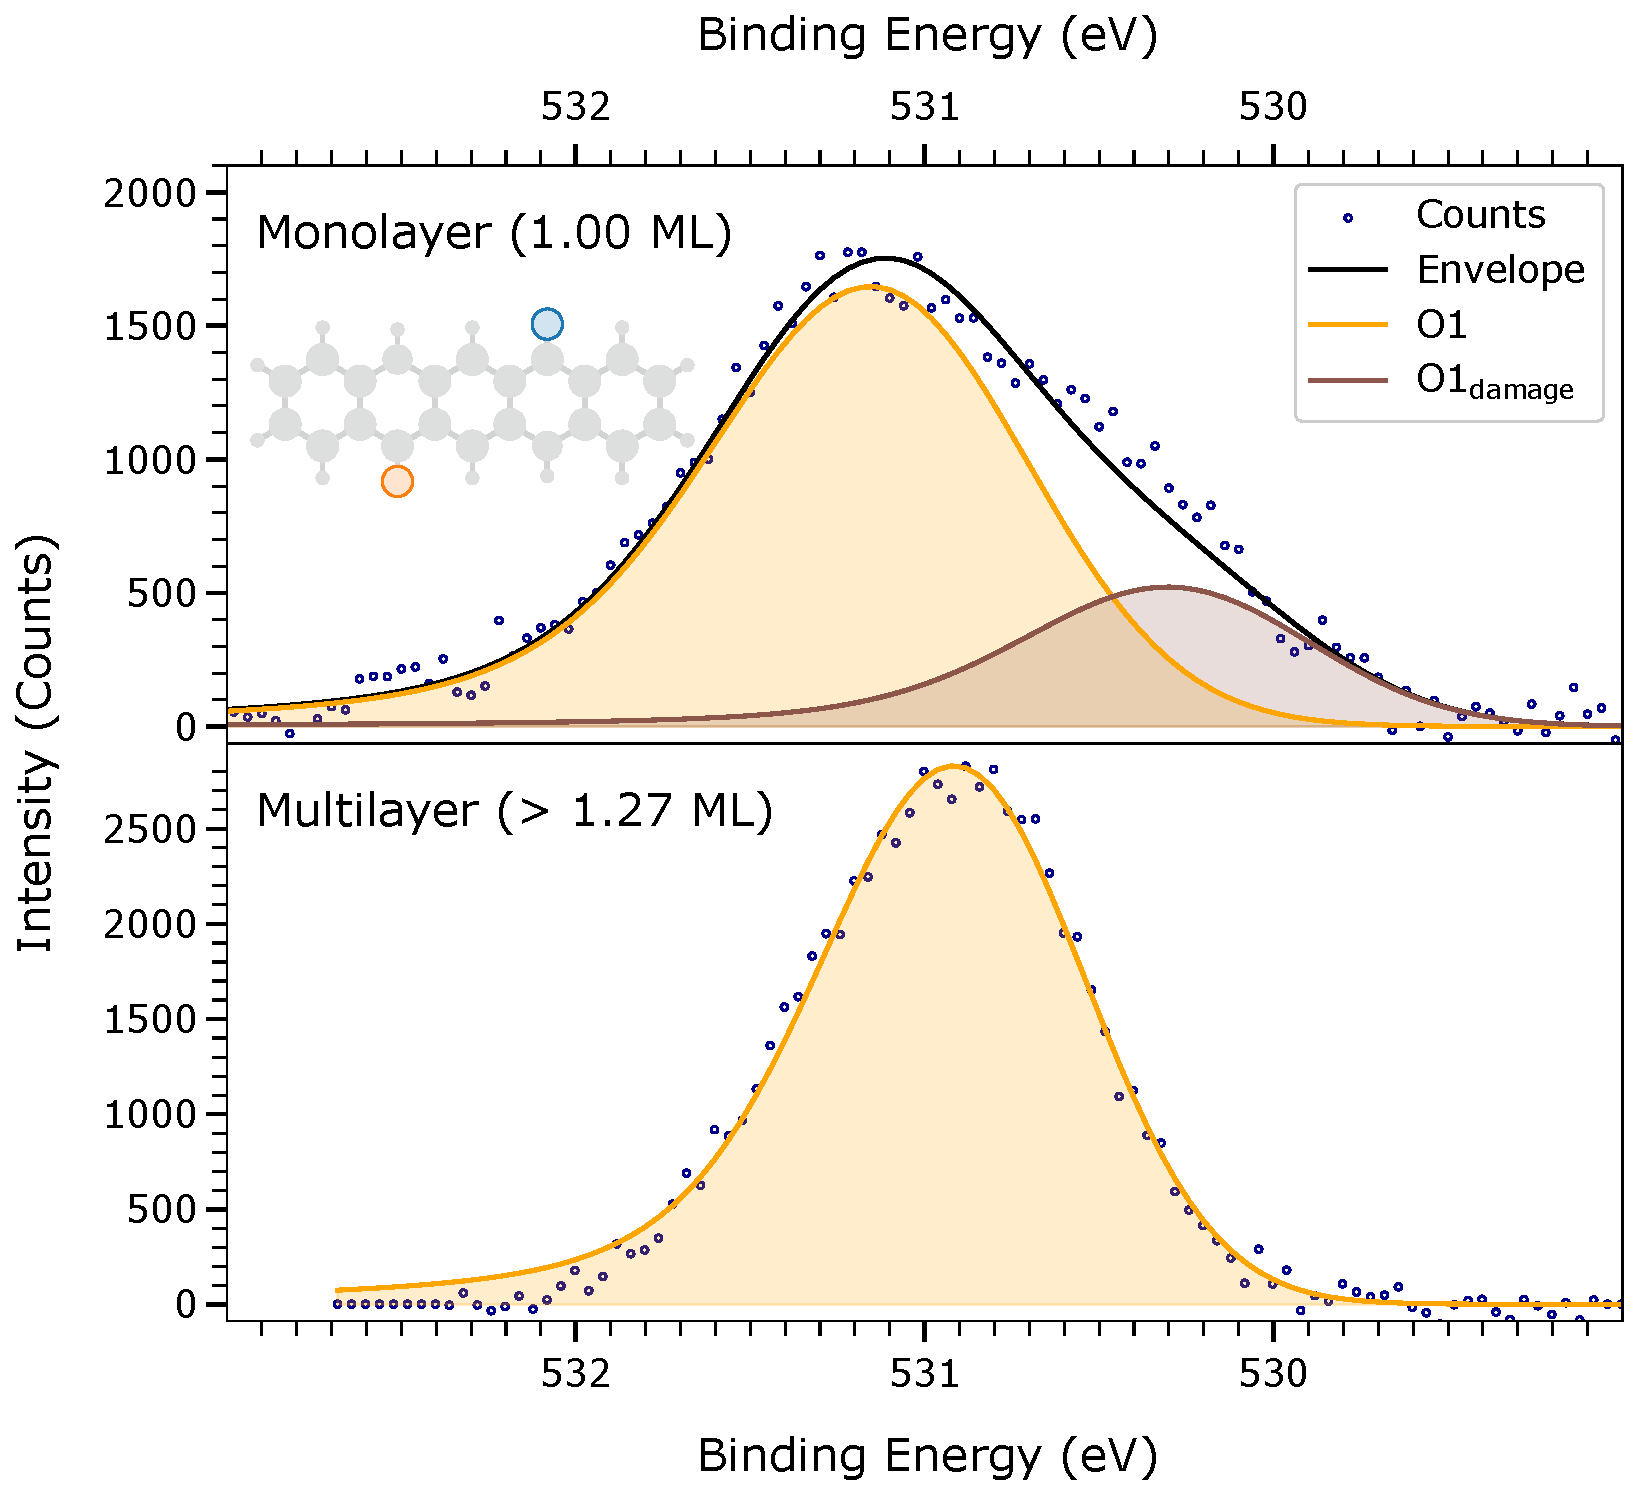
\includegraphics[width=\textwidth]{images/XPS/O1s-Multilayer.pdf}
	\caption{Comparison of the O1s \ac{XPS} spectra of \ac{QA} on the Ag(100) surface in the $\alpha$-phase for 1.00~\ac{ML} and 1.27~\ac{ML} coverage with the counts (blue circles), $\mathrm{O1}$ (yellow), $\mathrm{O1_{damage}}$ (brown) and the resulting envelope (black). The used fit parameters are summarized in \autoref{tab:XPS-O1s-Multilayer-fit}.}
	\label{fig:O1s-XPS-multilayer}
\end{figure}

The corresponding fit parameters for the O1s \ac{XPS} spectra of \ac{QA} on the Ag(100) surface in the $\alpha$-phase with both coverages are summarized in \autoref{tab:XPS-O1s-Multilayer-fit}.

\begin{table}[H]
	\centering
	\caption{\Ac{BE}, \ac{FWHM} and area ratio for the different peaks of the O1s \ac{XPS} spectra of \ac{QA} with a \ac{ML} and Multilayer coverage on the Ag(100) surface in the $\alpha$-phase.}
	\begin{tabular}{@{}ccccc@{}} \toprule
		 & peak & \ac{BE} (eV) & \ac{FWHM} (eV) & area ratio \\
		\midrule
		1.00~\ac{ML} & $\mathrm{O1}$ & 531.02 & 1.05 & 1 \\
		& $\mathrm{O1_{damage}}$ & 530.18 & 0.95 & - \\
        \midrule
		1.27~\ac{ML} & $\mathrm{O1}$ & 530.80 & 0.88 & 1 \\
		\bottomrule
	\end{tabular}
	\label{tab:XPS-O1s-Multilayer-fit}
\end{table}

The O1s \ac{XPS} spectrum of the \ac{QA} multilayer exhibits only one peak, which corresponds to the $\mathrm{O1}$ peak from the carbonyl groups. The \ac{BE} of this peak is 530.80~\si{eV}, which is 0.22~\si{eV} lower than the 1~\ac{ML} preparation. However, the \ac{FWHM} decreases from 1.05~\si{eV} to 0.88~\si{eV}. This is the same trend as observed for the N1s \ac{XPS} spectrum of the multilayer.

\newpage
\section{The phase transition}

\autoref{fig:XPS-C1s-phase-transition} shows the C1s \ac{XPS} spectra of \ac{QA} on the Ag(100) surface while heating the sample from room temperature ($\thicksim 300~\si{K}$) to 500~\si{K} to induce the phase transition from the $\alpha$- to the $\beta$-phase. The fit parameters from \autoref{tab:XPS-C1s-fit} were used for the individual peaks and the area ratio for the peaks of one phase were fixed.

\begin{figure}
	\centering
	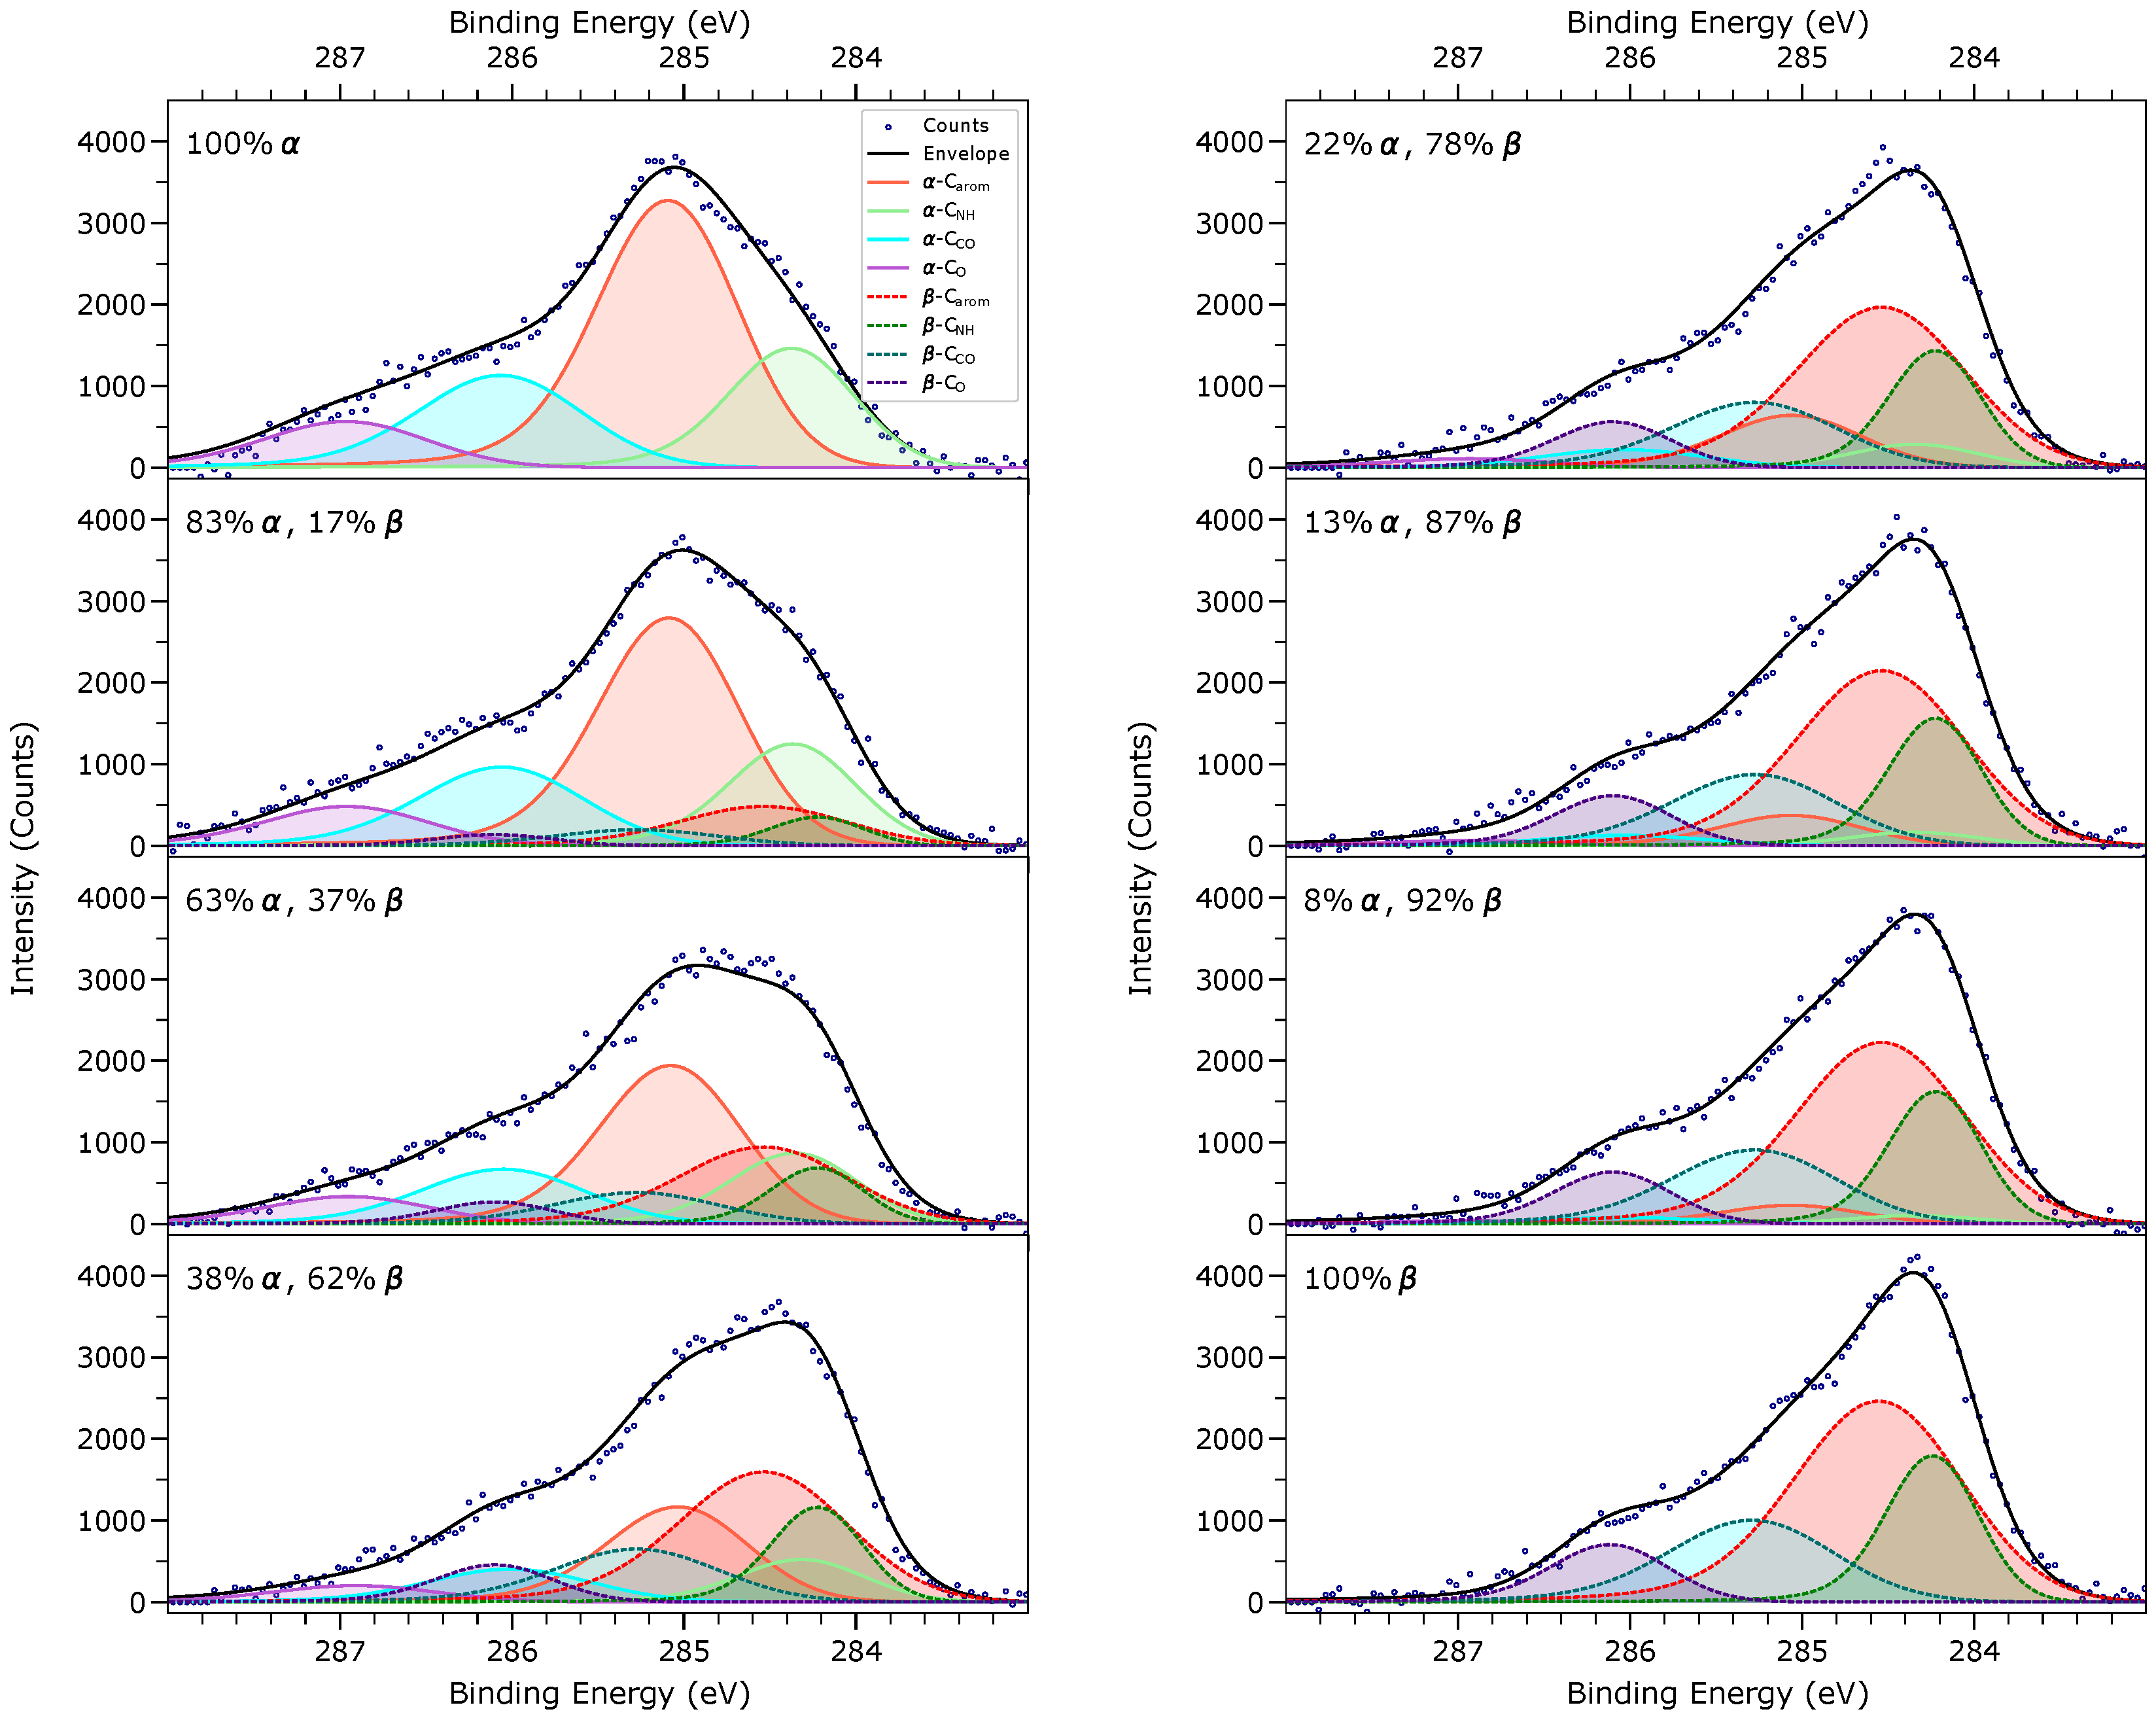
\includegraphics[height=\textwidth, angle=90]{images/XPS/C1s_Phase-Transition.pdf}
	\caption{C1s \ac{XPS} spectra of \ac{QA} on the Ag(100) surface while heating the sample from room temperature to 500~\si{K} to induce the phase transition from the $\alpha$- to the $\beta$-phase. The $\alpha$-phase peaks have solid lines, while the $\beta$-phase peaks have dashed lines. The fit parameters from \autoref{tab:XPS-C1s-fit} were used for the individual peaks and the area ratio for the peaks of one phase were fixed.}
	\label{fig:XPS-C1s-phase-transition}
\end{figure}

The C1s \ac{XPS} spectra in \autoref{fig:XPS-C1s-phase-transition} indicate the gradual phase transition from the $\alpha$- to the $\beta$-phase while heating the sample. The first spectrum at room temperature exhibits only the $\alpha$-phase peaks. With increasing temperature, the intensity of the $\beta$-phase peaks increases, while the intensity of the $\alpha$-phase peaks decreases. At the last \ac{XPS} spectrum at a temperature of 500~\si{K}, only the $\beta$-phase peaks are visible. This indicates that the phase transition is complete.

However, the exact temperature of the sample during the measurement is not known, as the sample temperature was only measured at the sample holder far away from the sample. Nevertheless, the phase transition can be clearly observed in the C1s \ac{XPS} spectra while heating the sample. 

Furthermore, it gives information about the underlying process of the phase transition. As the $\beta$-phase forms in a gradual manner while heating the sample, it indicates that the transition proceeds via domain-wise switching of the adsorbate phase.

\newpage
\section{XPS spectra of a damaged phase}

In contrast to the \ac{XPS} spectra of \ac{QA} on the Ag(100) surface in the $\beta$-phase, where the sample was successfully heated to induce the phase transition, \autoref{fig:XPS-C1s-Burnt} and \autoref{fig:XPS-N1s-Burnt} show the C1s and N1s \ac{XPS} spectra of a damaged \ac{QA} layer on the Ag(100) surface. Here, the sample was overheated to temperatures of approximately 600~\si{K}, which resulted in a damaged \ac{QA} layer instead of the formation of the $\beta$-phase.

The \ac{LEED} pattern of this damaged phase is shown in \autoref{fig:LEED-Burnt}. This pattern shows no ordered structure, indicating that the \ac{QA} layer is disordered due to the damage.

\begin{figure}[H]
	\centering
	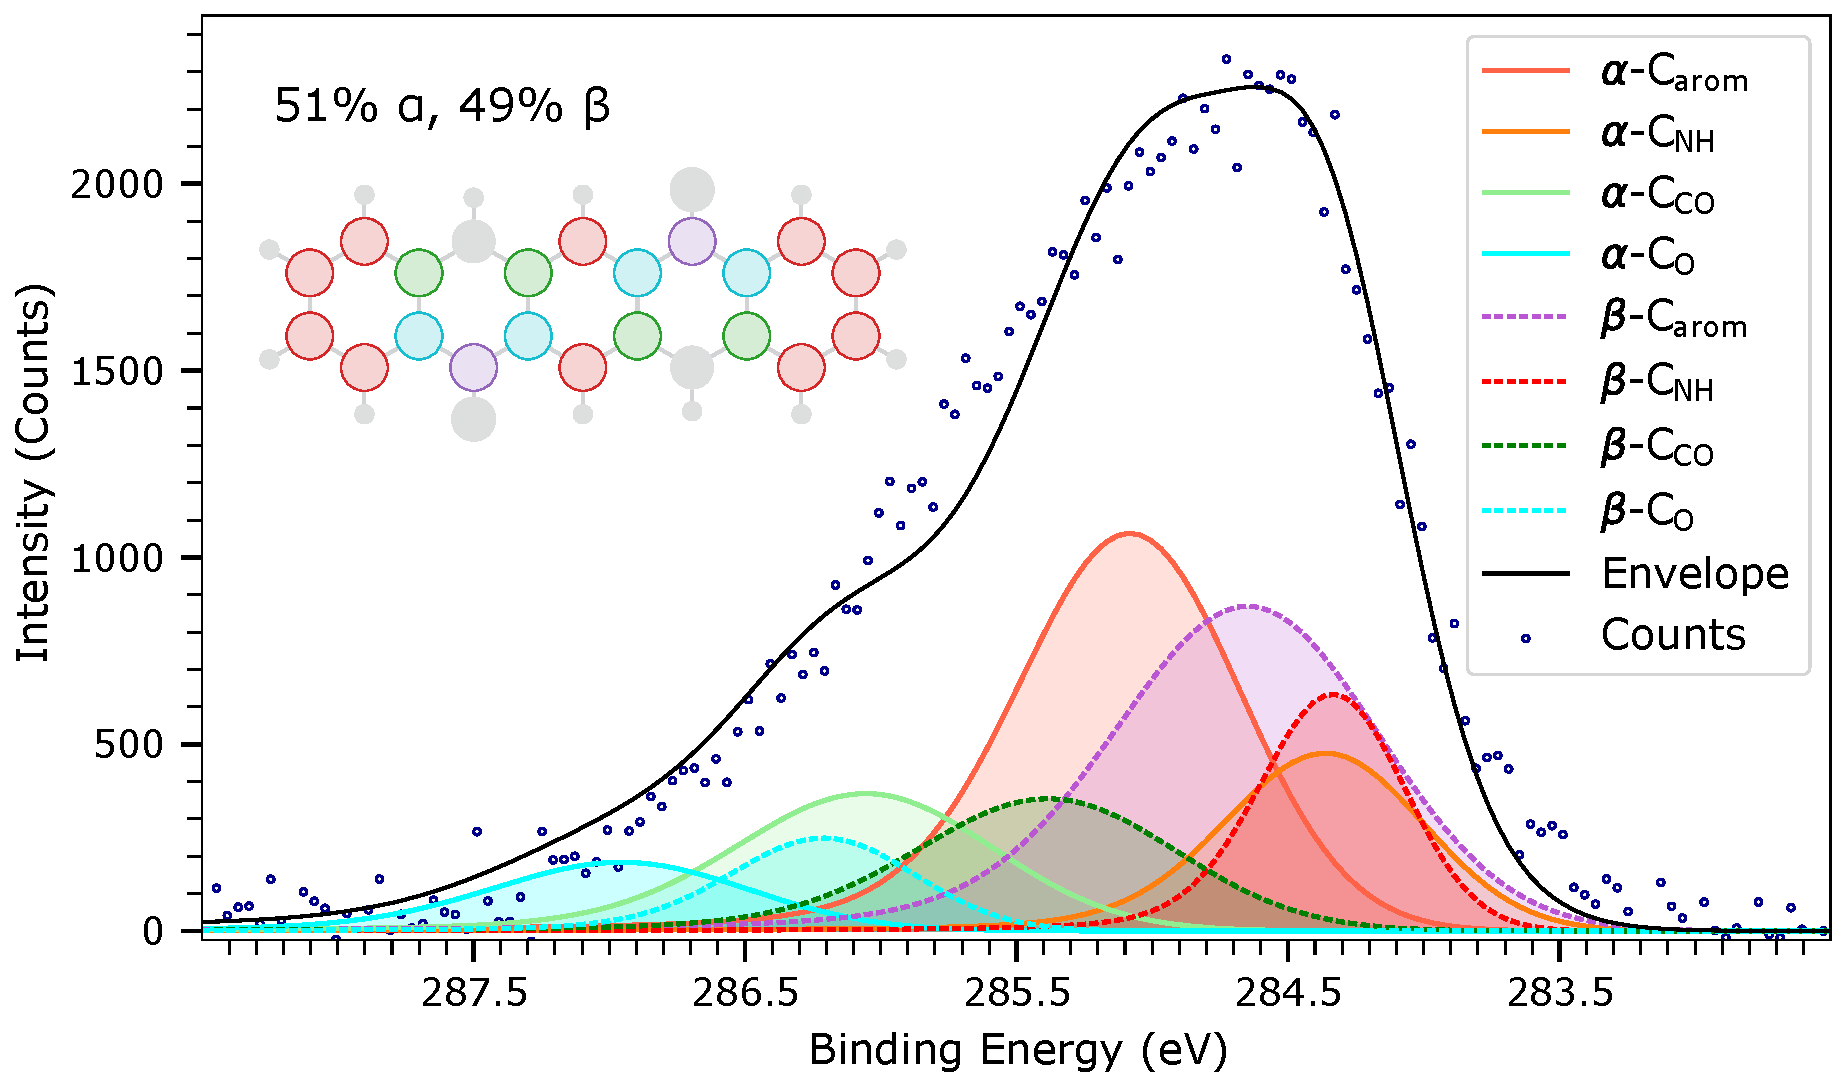
\includegraphics[width=\textwidth]{images/XPS/C1s-BurntPhase.pdf}
	\caption{C1s \ac{XPS} spectra of a damaged \ac{QA} layer on the Ag(100) surface.}
	\label{fig:XPS-C1s-Burnt}
\end{figure}

Even though the \ac{LEED} pattern shows no ordered structure, the C1s \ac{XPS} spectrum in \autoref{fig:XPS-C1s-Burnt} is fitted with an 50:50 ratio of the $\alpha$- and $\beta$-phase peaks from \autoref{tab:XPS-C1s-fit}. The fit describes the experimental data very well, indicating that both phases are still present in the damaged layer. 

This indicates that the damage of the \ac{QA} molecules on the Ag(100) surface does not lead to a desorption of the molecules, but rather to a loss of the long-range order in the layer. Nevertheless, the chemical environment of the \ac{QA} molecules remains analogous to a combination of the intact $\alpha$- and $\beta$-phase.

\autoref{fig:XPS-N1s-Burnt} shows the N1s \ac{XPS} spectrum of the same damaged \ac{QA} layer on the Ag(100) surface.

\begin{figure}[H]
	\centering
	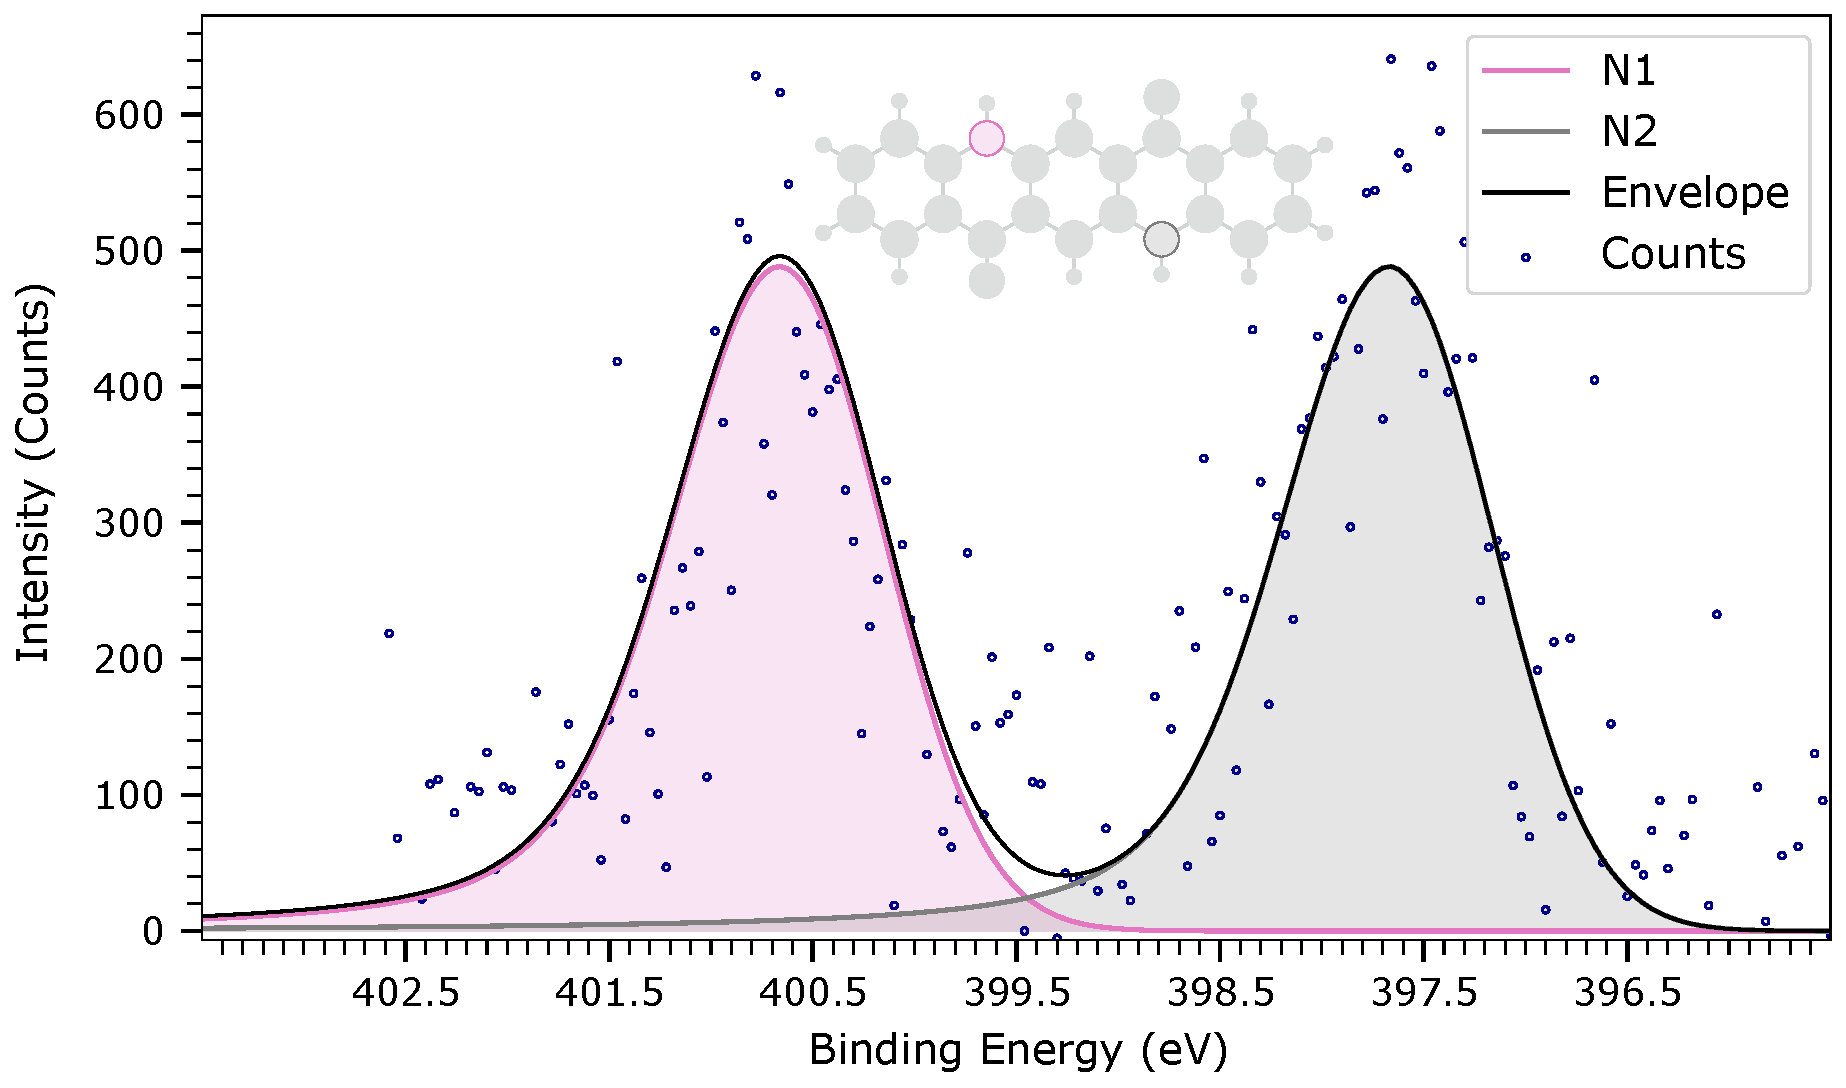
\includegraphics[width=\textwidth]{images/XPS/N1s-BurntPhase.pdf}
	\caption{N1s \ac{XPS} spectra of a damaged \ac{QA} layer on the Ag(100) surface.}
	\label{fig:XPS-N1s-Burnt}
\end{figure}

In contrast to the C1s \ac{XPS} spectrum, the N1s \ac{XPS} spectrum in \autoref{fig:XPS-N1s-Burnt} is fitted only with the $\beta$-phase peaks, where the area ratio of the $\mathrm{N1}$ and $\mathrm{N2}$ peak is 1:1. Furthermore, the difference in \ac{BE} between the $\mathrm{N1}$ and $\mathrm{N2}$ peak increases from 2.21~\si{eV} in the intact $\beta$-phase to 2.99~\si{eV} in the damaged layer. This indicates that the chemical environment of the N atoms in the damaged layer differs more significantly compared to the intact $\beta$-phase.

Even though the N1s \ac{XPS} spectrum of the damaged layer exhibits two distinct peaks, the exact \ac{BE} and area ratio of these peaks may be not precisly determined due to the low intensity of the N1s signal. This is clearly visible in the high noise level of the experimental data in \autoref{fig:XPS-N1s-Burnt}.

\cleardoublepage